\documentclass[12pt,twoside,letterpaper]{article}

\topmargin -0.25cm
\textwidth 15.5cm
\textheight 22cm
\oddsidemargin 0.5cm
\evensidemargin 0.5cm


%\usepackage{epsfig,rotating}
\usepackage{amssymb}
\usepackage{amsmath}
\usepackage{graphicx}
\usepackage{epstopdf}
\usepackage[figuresright]{rotating}
\usepackage{verbatim}
\usepackage[section] {placeins}
\usepackage{multirow}

%\usepackage{doublespace}

\usepackage{setspace}

\newcommand{\vbb}{0\nu\beta\beta}
\newcommand{\vvbb}{2\nu\beta\beta}
\newcommand{\Te}{^{130}Te}
\newcommand{\Se}{^{82}Se}
\newcommand{\B}{^{8}B}
\newcommand{\Bten}{^{10}B}
\newcommand{\Cten}{^{10}C}

\usepackage{lineno}
\linenumbers

\begin{document}

\vspace*{-3.5cm}
\begin{flushright}
Draft for NIMA\\
version 5\\
\today
\end{flushright}

%\vspace{0.25in}

%\tableofcontents
%\newpage

\begin{center}
  \begin{Large}
%  {\bf Double-beta decay event topology reconstruction using fast photo-detector in a kiloton-scale liquid scintillator detectors}
  {\bf Separating double-beta decay events from solar neutrino interactions in kiloton-scale liquid scintillator detectors}
  \end{Large}
\end{center}

%\vspace{0.25in}

\begin{center}
Andrey Elagin$^1$, Henry Frisch$^1$, Lindley Winslow$^2$, $et$ $al$ {\bf (opt-in)}\\
\emph{$^1$Enrico Fermi Institute, University of Chicago\\ 
$^2$Massachusetts Institute of Technology}
\end{center}

\setstretch{1.5}


\begin{abstract}
We propose a technique for separating $\vbb$-decay events from background due to $\B$ solar neutrino interactions in a liquid scintillator detector. The technique compares event topology of the signal and background events using spherical harmonics analysis of the early light emitted in $\vbb$-decay and $\B$ events. Selection of early photons using fast photo-detectors allows for separation of directional Cherenkov from isotropic scintillation light and identification of two event topologies based on the spatial distribution of the early photons in the detector.
\end{abstract}

\newpage
\tableofcontents
\newpage





\section{Introduction}

{\bf Introductory paragraph saying that $\vbb$-decay is important and we'd like to improve sensitivity of liquid scintillator detectors.}

{\bf Another paragraph saying that this is a follow up on our preceding paper~\cite{Directionality}}
  
As have been shown in~\cite{Directionality} photo-detectors with time resolution of $\sim$100~ps can allow for selection of photons that contain significant fraction of Cherenkov light produced by 1-5~MeV electrons in a kilo-ton scale liquid scintillator detector.

\begin{figure}[htb]
\centering
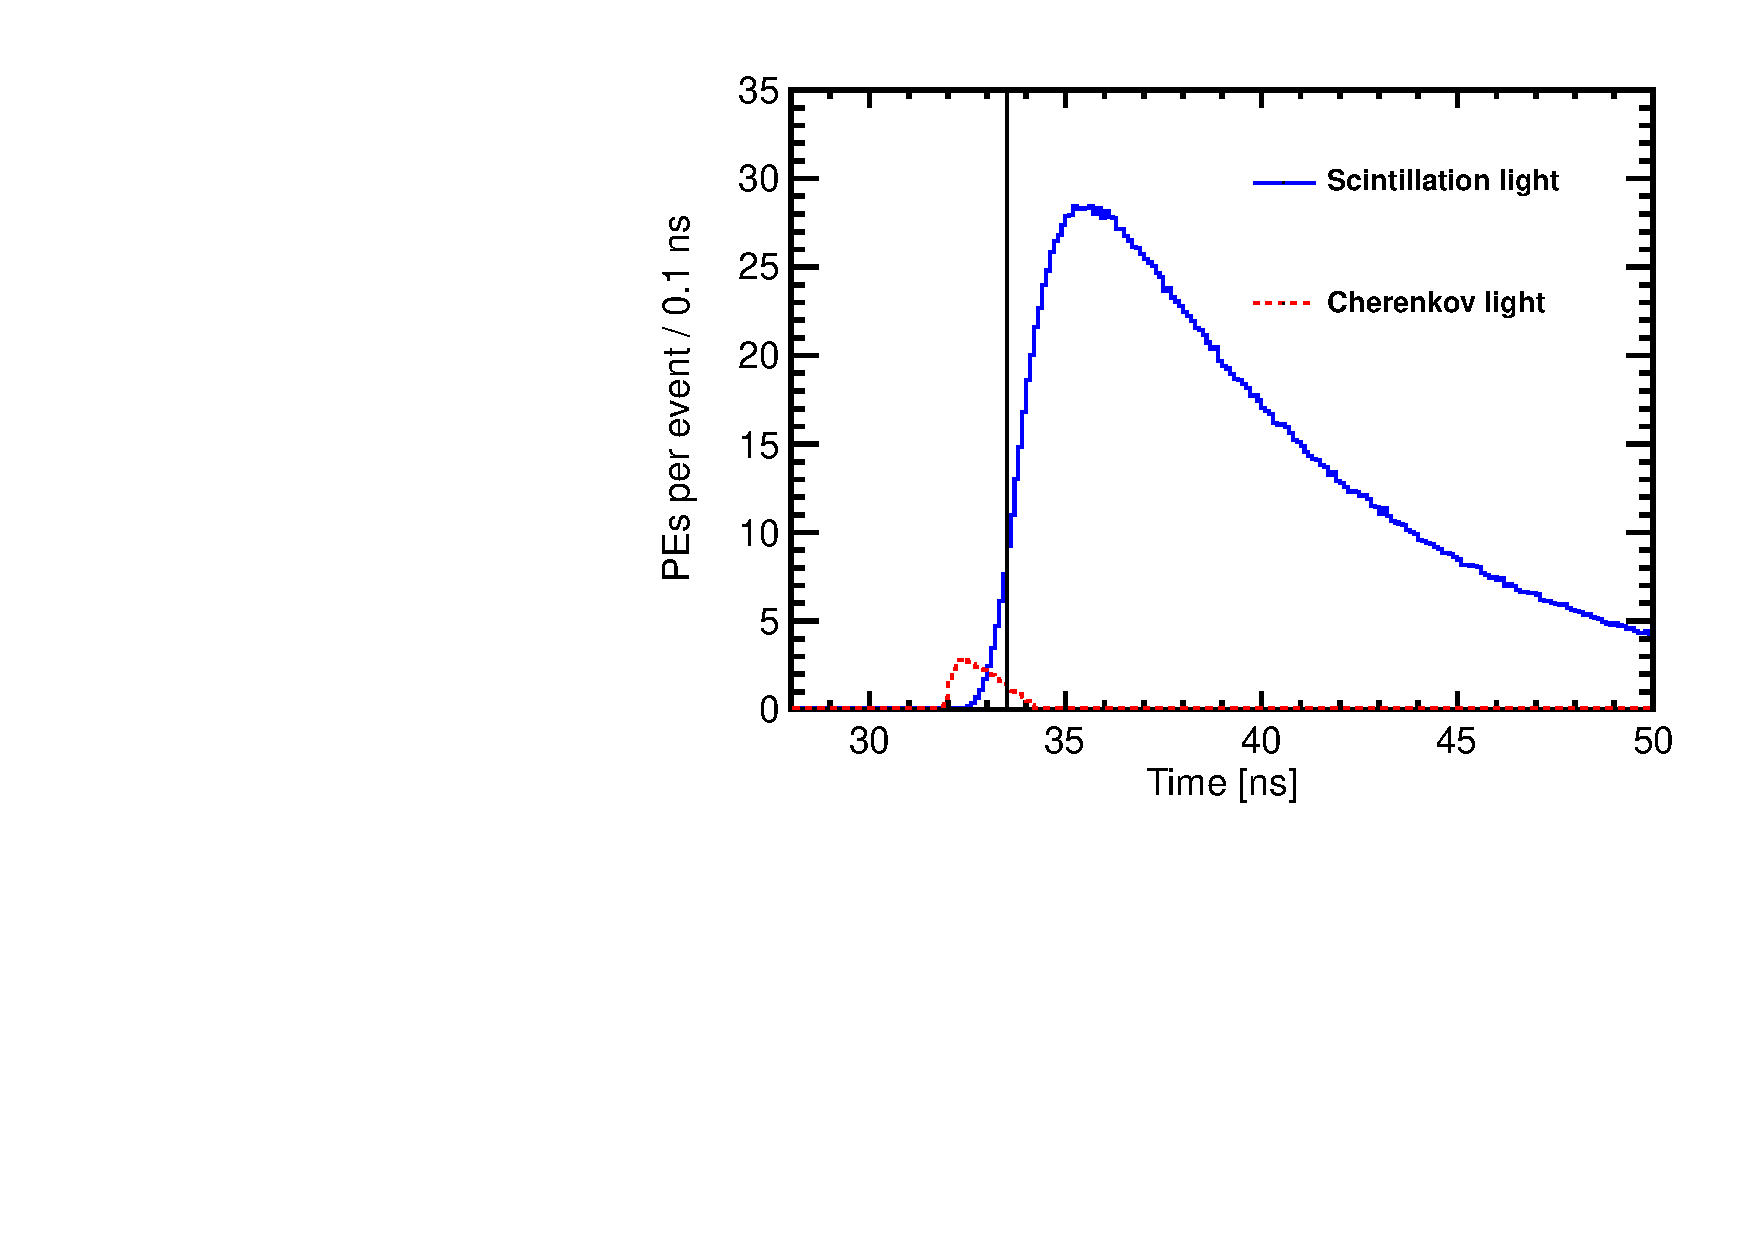
\includegraphics[angle=0,width=0.45\textwidth]{plots/hT_Te130.pdf}
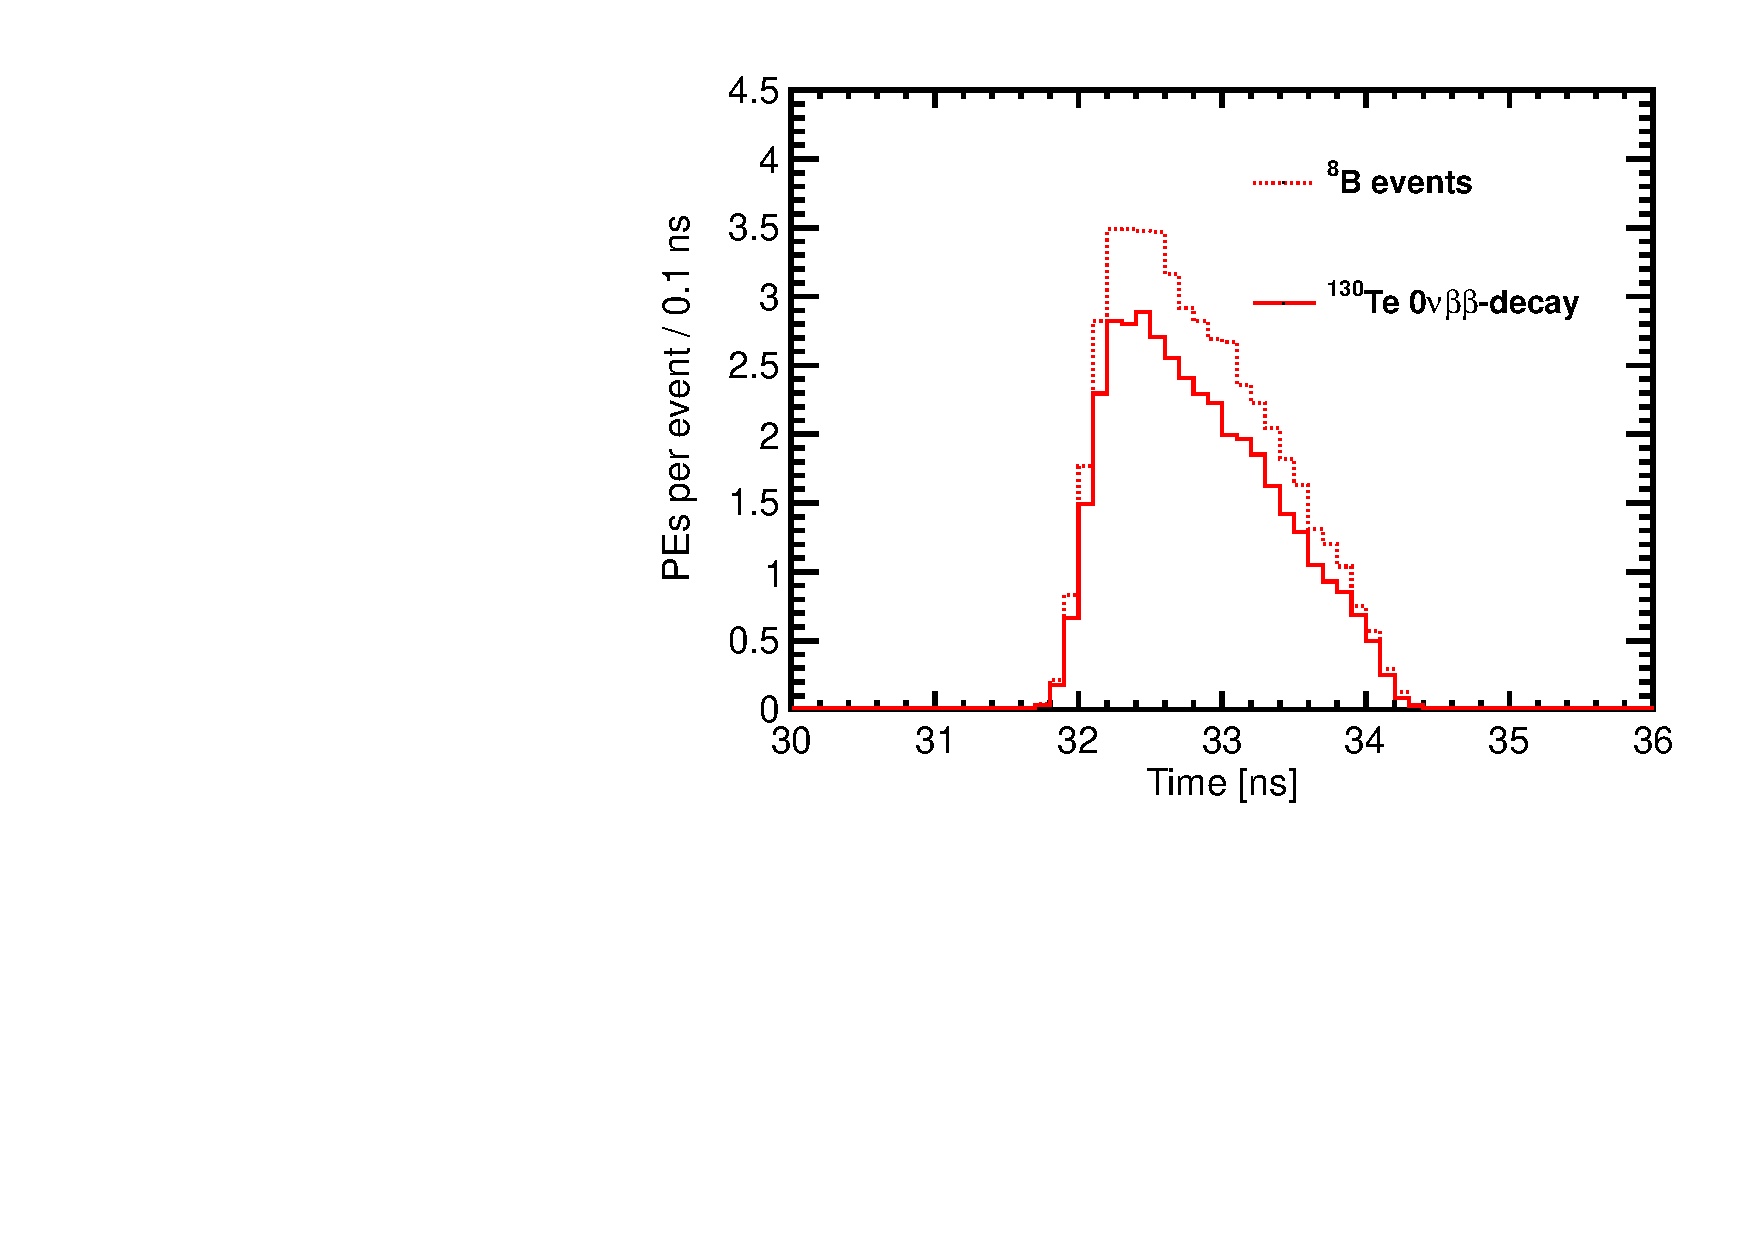
\includegraphics[angle=0,width=0.45\textwidth]{plots/hTche_Te130_B8.pdf}
\caption{(Left) Photo-electron (PE) arrival times after application of the photo-detector transit time spread (TTS) of 100~ps for the simulation of 1000 $\vbb$-decay events of $\Te$ at the center of the detector. PEs from Cherenkov light (red, dash line) and scintillation light (blue, solid
line) are compared. The black vertical line illustrates a time cut at 33.5 ns. (Right) Comparison between Cherenkov PEs arrival time for $\Te$ $\vbb$-decay (solid line) and $\B$ (dotted line) events. {\bf Distributions of the scintillation PEs arrival time are indistinguishable between $\Te$ $\vbb$-decay and $\B$ due to identical total energy in the event, Q($\Te$)$=$2.529~MeV.} }
\label{fig:Arrival_time}
\end{figure}


\begin{figure}[htb]
\centering
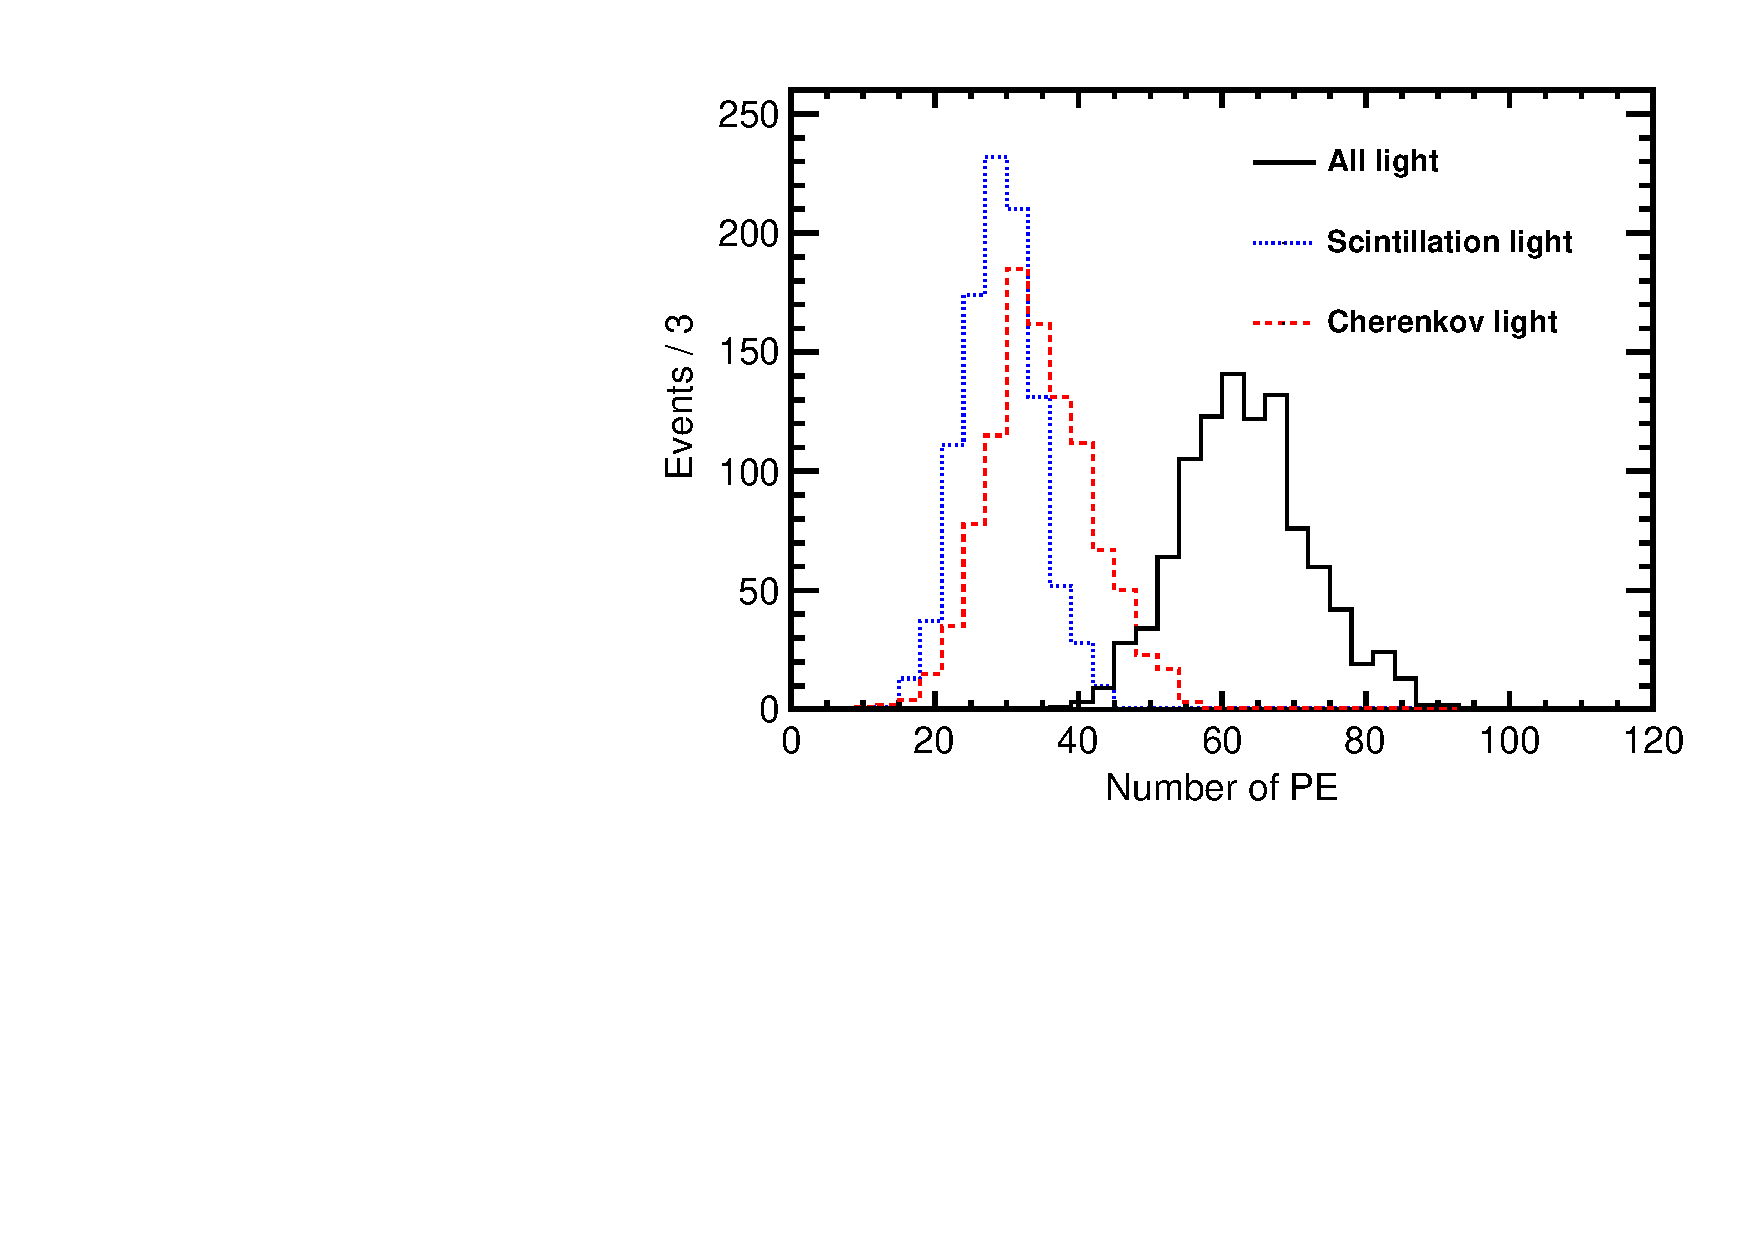
\includegraphics[angle=0,width=0.45\textwidth]{plots/hMomNPhot_Te130.pdf}
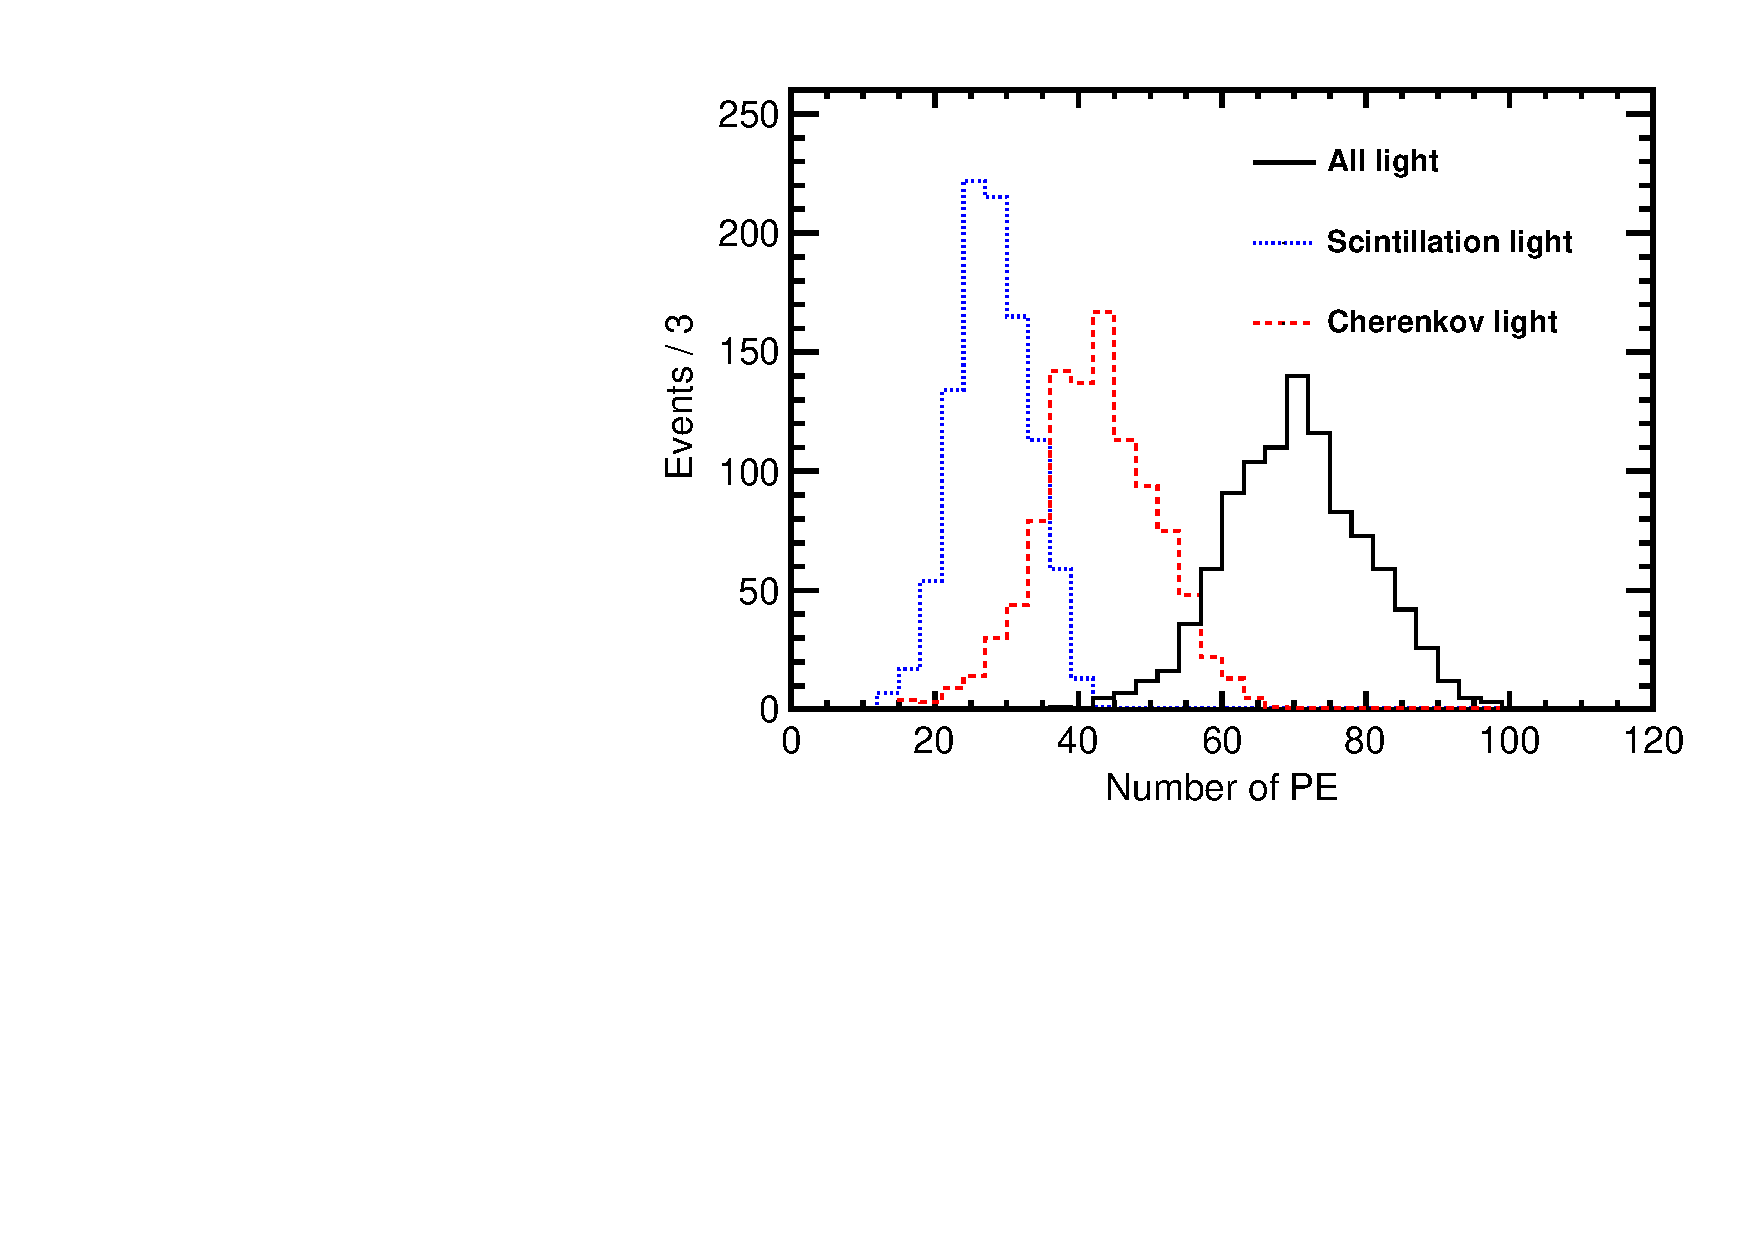
\includegraphics[angle=0,width=0.45\textwidth]{plots/hMomNPhot_1el_2p529MeV.pdf}
\caption{Number of Cherenkov (red dash line), scintillation (blue dotted line), and total (black solid line) PEs for the simulatio of 1000 $\Te$ $\vbb$-decay (left panel) and $\B$ (right panel) events.}
\label{fig:NPhot}
\end{figure}


\section{Discussion on backgrounds}
In a large liquid scintillator detector two dominant backgrounds to $\vbb$-decay signal are $\vvbb$-decay and QE interactions of $\B$ solar neutrinos. As an example we show comparison between signal and various backgrounds for SNO+ experiment in Fig.~\ref{fig:SNOp_bkgs}.


\begin{figure}[htb]
\centering
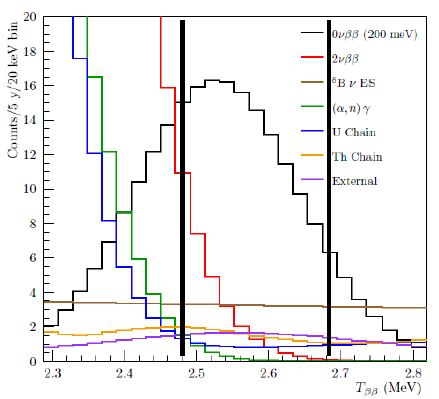
\includegraphics[angle=0,width=0.75\textwidth]{plots/SNOp_backgrounds.JPG}
\caption{SNO+ Phase I signal and background energy spectrum (visible kinetic energy reconstructed under a $\vbb$ hypothesis). Plot taken from~\cite{SNOp_paper}}
\label{fig:SNOp_bkgs}
\end{figure}


Figure~\ref{fig:Kinematics} shows kinematics of $\vbb$- and $\vvbb$-decays.  In the region of interest (ROI) where total kinetic energy of the electrons is close to the energy spectrum end point, Q-value, there is no difference in kinematics of $\vbb$- and $\vvbb$-decays. Therefore the energy resolution is the key detector parameter to discriminate between $\vbb$- and $\vvbb$-decays.

\begin{figure}[htb]
\centering
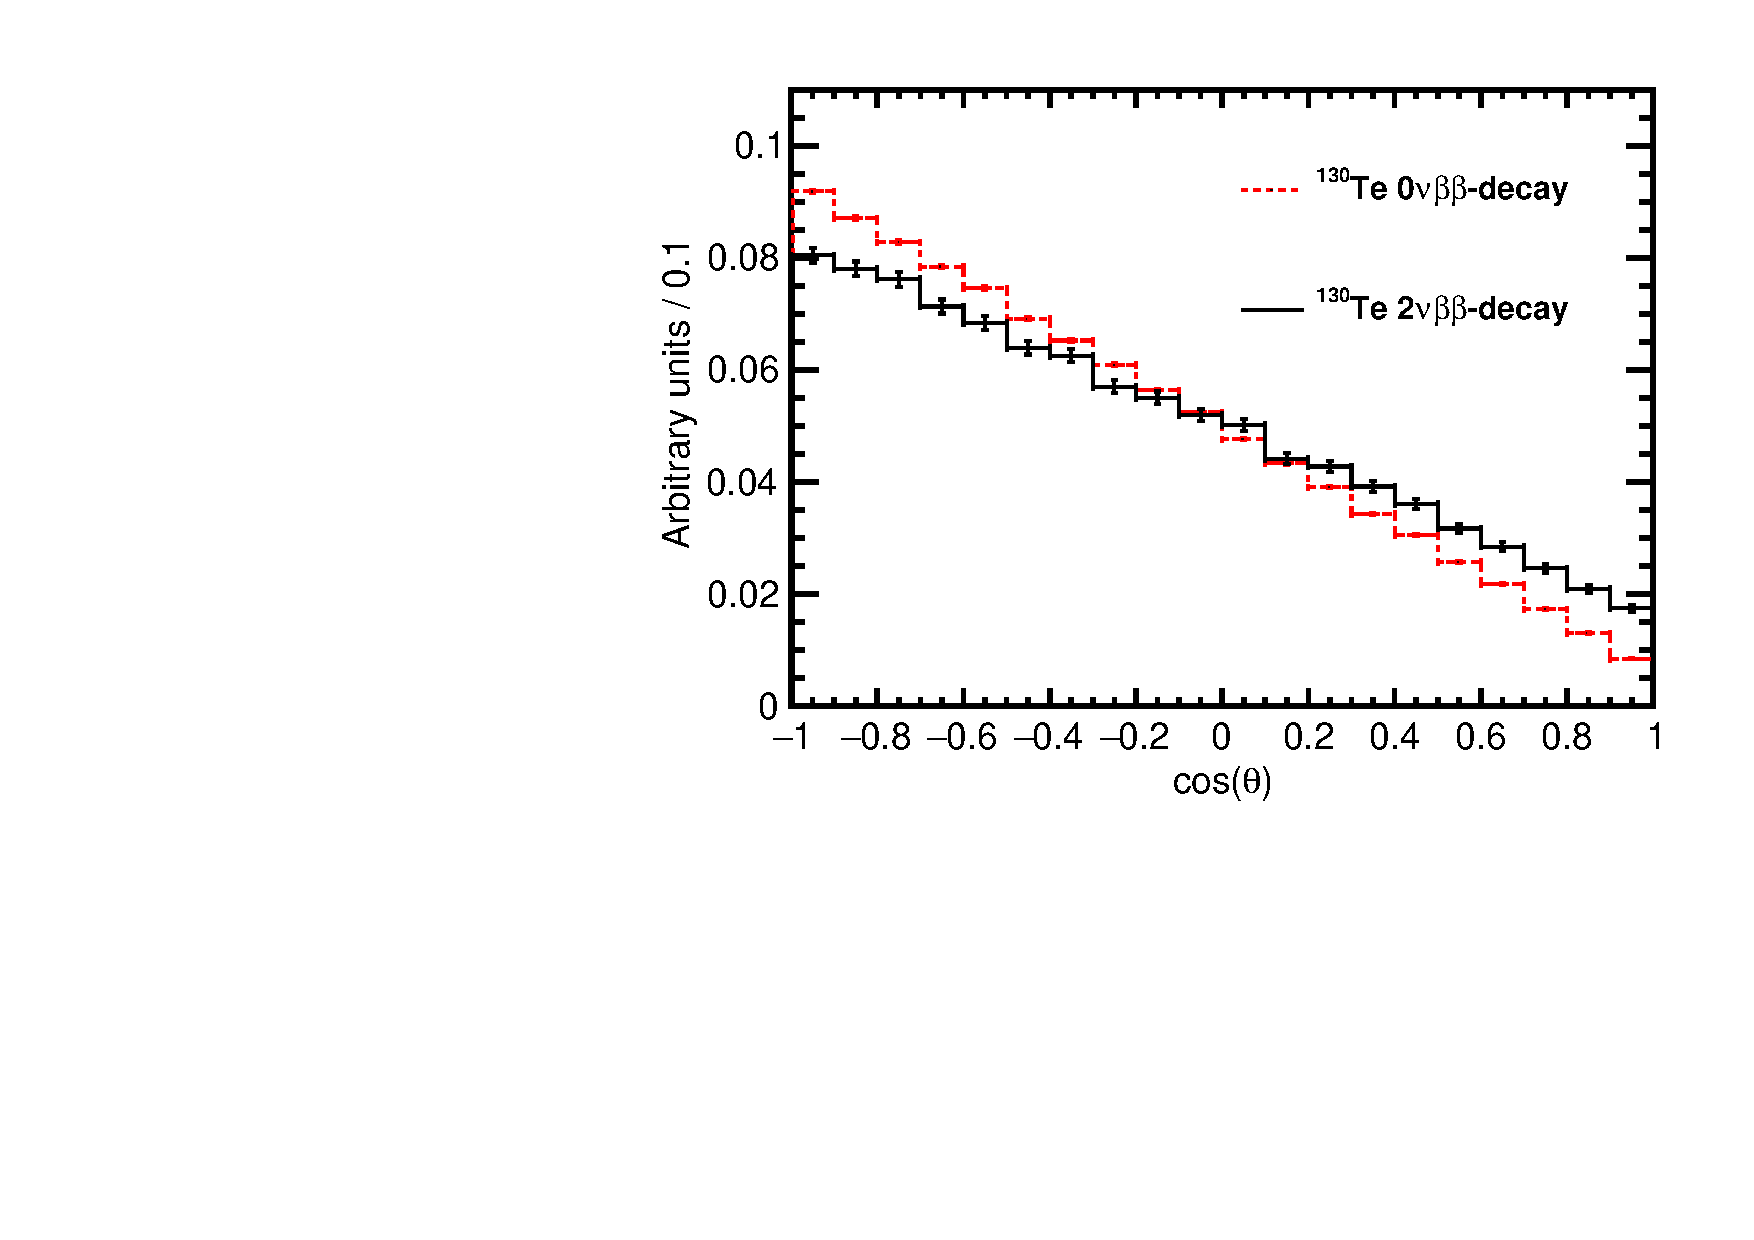
\includegraphics[angle=0,width=0.49\textwidth]{plots/hCos_Te130.pdf}
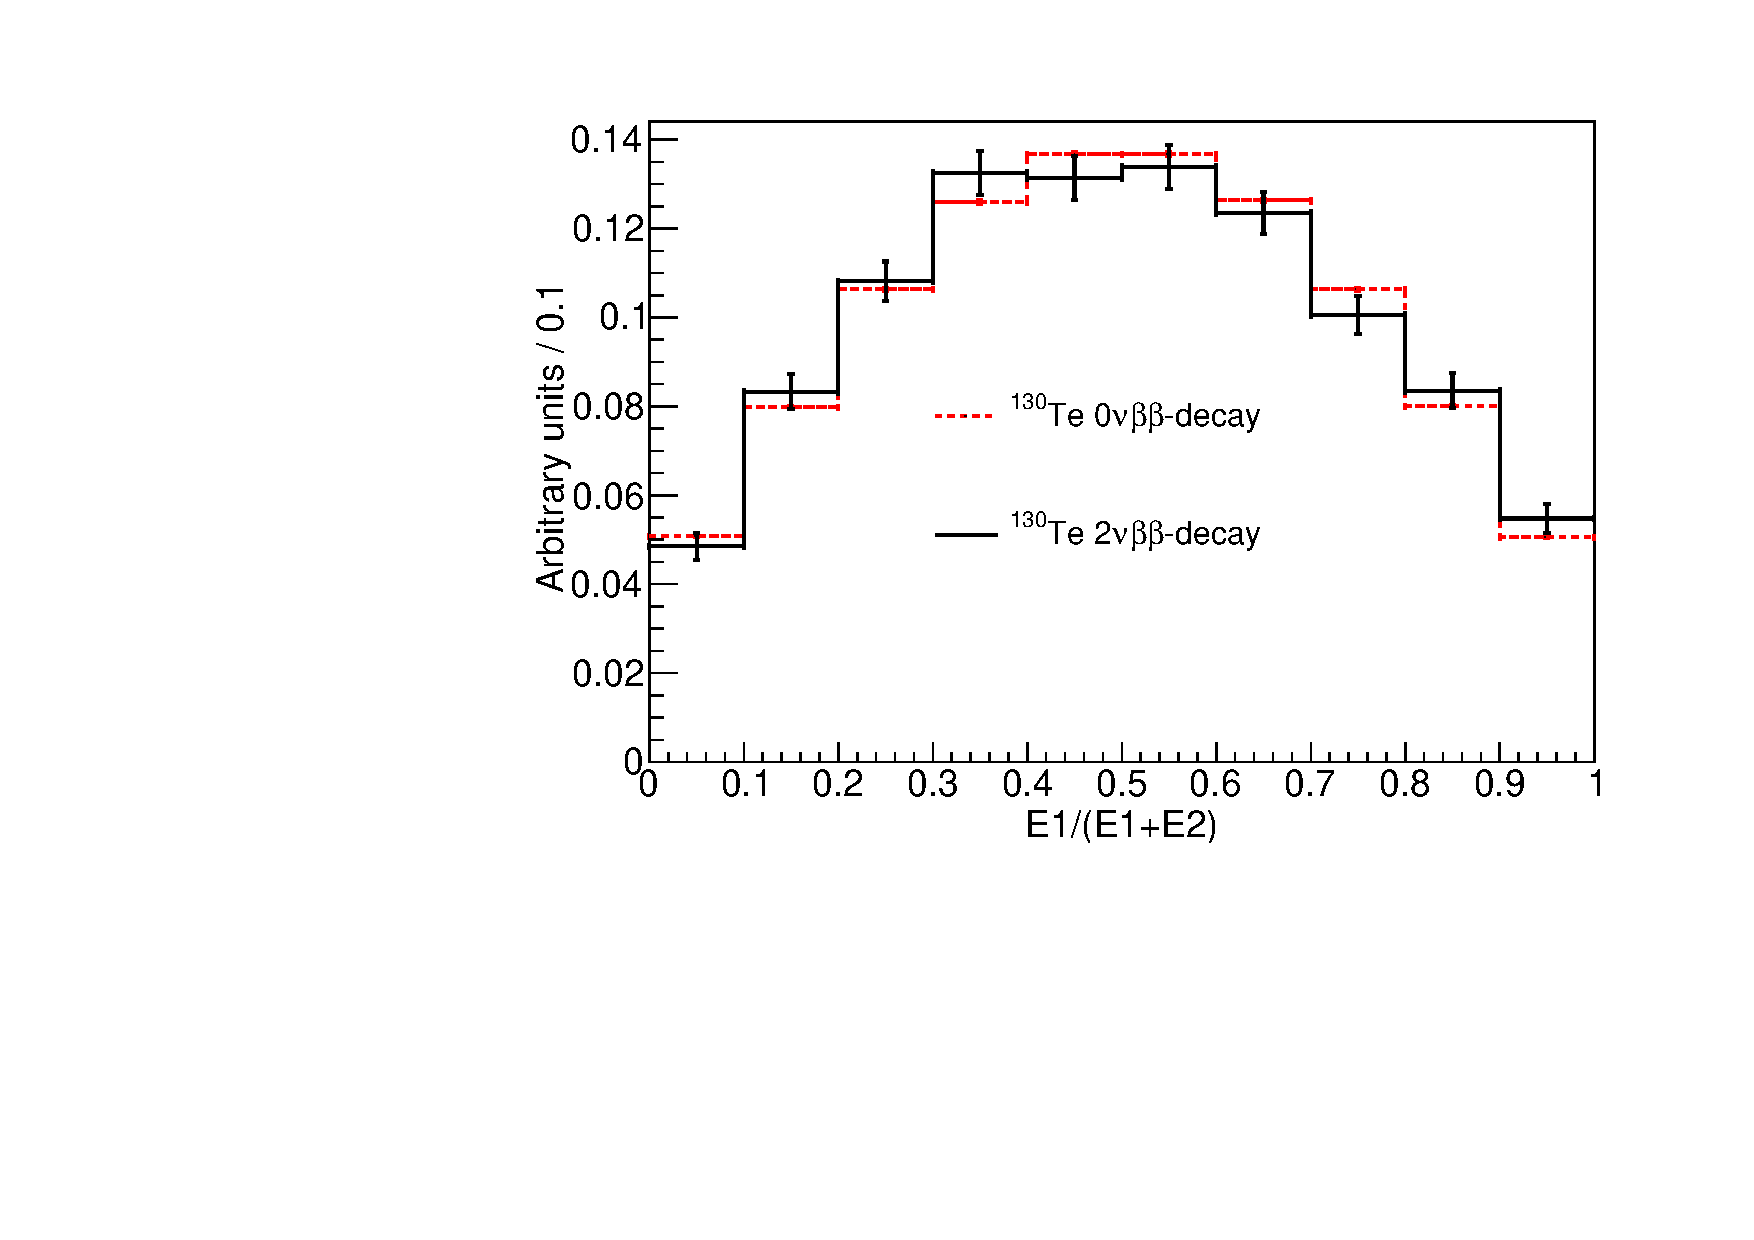
\includegraphics[angle=0,width=0.49\textwidth]{plots/hE1toQ_Te130.pdf}
\caption{Comparison between kinematics of $\vbb$- (dashed red lines) and $\vvbb$-decays (solid black lines) for events with the total kinetic energy of the electrons above 90\% of the Q-value. (Left) Cosine of the angle between two electrons. (Right) Fraction of energy carried by one of the two electrons. Due to limited statistic around the energy spectrum end point for $\vvbb$-decay we show statistical errors for each bin.}
\label{fig:Kinematics}
\end{figure}


While the $\vvbb$-decay is topologically very similar to the $\vbb$-decay signal the next largest background coming from the $\B$ solar neutrino interactions result in one electron that leads to a distinct pattern of the Cherenkov photons.

\section{Description of the detector geometry and simulation}
{\bf Details are in~\cite{Directionality}. Only one or two paragraphs here.}

\section{Event Topology and Spherical Harmonics}
Signature of the $\vbb$-decay is two electrons with total kinetic energy equal to the isotope Q-value (e.g., 2.529~MeV for $\Te$). These two electrons are often above Cherenkov threshold and therefore will produce two (fuzzy) rings of Cherenkov light on top of isotropic scintillation light. $\B$ background events have only one electron producing one Cherenkov ring.

In the detector regions where Cherenkov and scintillation light overlap the Cherenkov light on average arrives earlier due to a time delay in emission and a shorter wavelengths of the scintillation light. Therefore, while a vast majority of light produced in $\vbb$-decay events consists of scintillation photons, timing information can be used to select a sample of photons with high fraction of Cherenkov light.

Due to directional nature of the Cherenkov light the spatial distribution of early photons on the detector sphere will be different for the $\vbb$-decay signal and the background from $\B$ events. Figure~\ref{fig:EvtDisplay} shows event displays of $\Te$ $\vbb$-decay signal events and $\B$ background. For quantitative description of the difference in the event topology we analyze spherical harmonics of the photon distributions on the detector sphere. We construct rotation invariant variables and compare them between signal and background events.

The simplest case for spherical harmonics analysis are events with the vertex located exactly in the center of the detector. For such event Cherenkov and scintillation light can be separated by applying a time cut on the photon arrival time as demonstrated in~\cite{Directionality}. To introduce the technique of spherical harmonics analysis we will follow the same strategy as in~\cite{Directionality} and use central events with a slightly different cut on the photon arrival time of 33.5~ns.



\begin{figure}[htb]
\centering
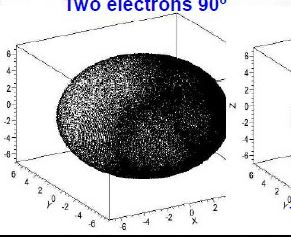
\includegraphics[angle=0,width=0.49\textwidth]{plots/EvtDisplay_two_electrons.JPG}
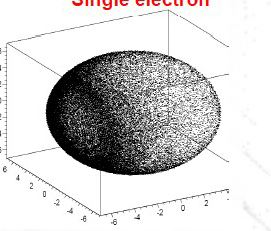
\includegraphics[angle=0,width=0.49\textwidth]{plots/EvtDisplay_one_electron.JPG}
\caption{Examples of PEs position on the detector sphere after time cut of 33.5ns. PEs from Cherenkov (red) and scintillation light (blue) are compared. (Left) PEs from two electrons produced in an event of $\vbb$-decay of $\Te$. In this event the angle between the electrons is $\sim$90$^o$ and the electrons energies are A.B~MeV and D.C~MeV. (Right) PEs from one electron produced in an event of $\B$ solar neutrino interaction. In this event the electron energy is E.F~MeV.}
\label{fig:EvtDisplay}
\end{figure}

\subsection{Mathematical description of spherical harmonics analysis}
A function $f(\theta,\phi)$ can be decomposed to a sum of spherical harmonics:

\begin{eqnarray}
\label{eq1}
f(\theta,\phi) = \sum_{l=0}^{\infty} \sum_{m=-l}^{l} f_{lm} Y_{lm}(\theta,\phi),
\end{eqnarray}

where $Y_{lm}$ are Laplace's spherical harmonics defined in Eq.~\ref{eq2} in real-value basis using Legendre polynomials $P_l$. Coefficients $f_{lm}$ are defined in Eq.~\ref{eq3} 

\begin{eqnarray}
\label{eq2}
Y_{lm} = LONGformulaHERE
\end{eqnarray}

\begin{eqnarray}
\label{eq3}
f_{lm} = LONGformulaHERE
\end{eqnarray}

Equation~\ref{eq4} defines multiple moments $S_l$ which are invariant under rotation. Combination of $S_l$'s for ($l$=0,1,2...) is determined by the event topology and can be used to distinguish between different topologies.

\begin{eqnarray}
\label{eq4}
S_l = \sum_{m=-l}^{m=l} |f_{lm}|^2
\end{eqnarray}

Figure~\ref{fig:Moments} compares $S_l$ distributions for two electrons emitted at 180 degree, two electrons at 90 degree, and a single electron. Total kinetic energy of the electrons is the same in all three cases.


\begin{figure}[htb]
\centering
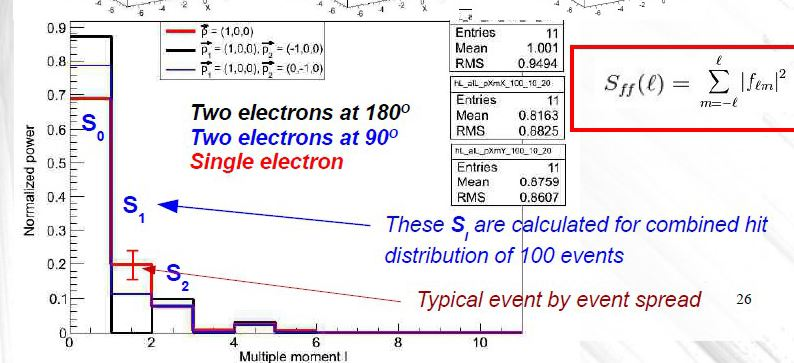
\includegraphics[angle=0,width=0.95\textwidth]{plots/Multiple_moment.JPG}
\caption{Average S$_l$ values for two electrons at 180 degree (color1) and 90 degree (color2) 1.5~MeV each and a single electron (color3) with the energy of 3~MeV. Error bars are RMS values of each corresponding individual S$_l$ distribution (each consists of 1000 events simulated at the center of the detector) indicating typical event-by-event variation.}
\label{fig:Moments}
\end{figure}


In order to compare spherical harmonics for events with vertices located off-center anywhere inside the detector volume a coordinate transformation for each photon hit is needed. The transformation applied for each photon hit within an event is shown in Fig.~\ref{fig:SphH_transform}. Solid circle schematically shows actual detector boundaries. Dotted circle shows a new sphere of radius R$=$6.5~m with the event vertex position in the center. The radius vector of each photon hit is stretched or shorten until intersection with this new sphere using transformation $\vec{r}^{,}_{hit} = \frac{\vec{a}}{|\vec{a}|} \cdot R$. Where $\vec{r}^{,}_{hit}$ is a new radius vector of the photon hit, R is detector sphere radius, and $\vec{a}=\vec{r}_{hit} - \vec{r}_{vtx}$ with $\vec{r}_{hit}$ and $\vec{r}_{vtx}$ being radius vectors of the photon hit and vertex position in original coordinates.

\begin{figure}[htb]
\centering
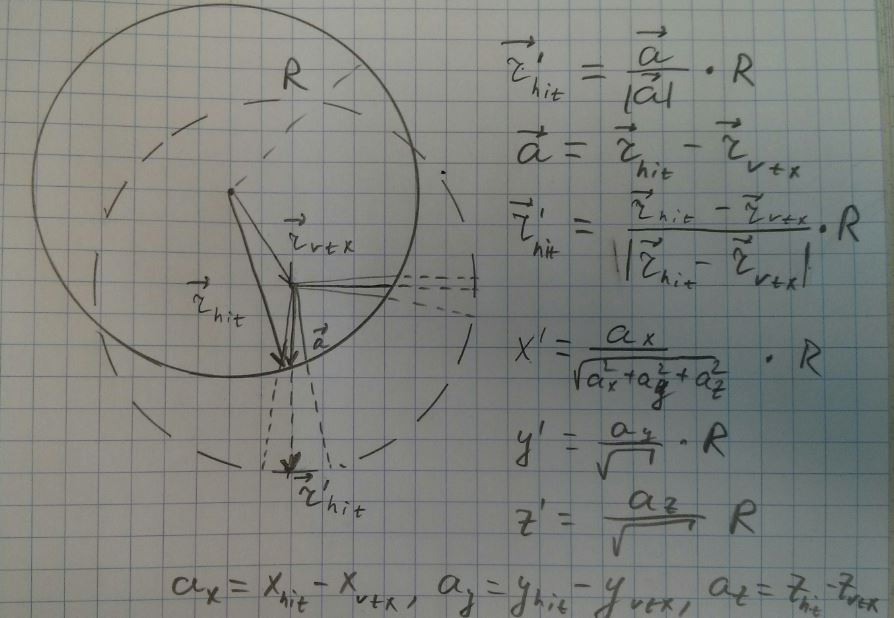
\includegraphics[angle=0,width=0.95\textwidth]{plots/SphH_transform_sketch.JPG}
\caption{Coordinate transformation applied to events that are off-center. Solid circle schematically shows actual detector boundaries. Dotted circle shows a new sphere of radius R$=$6.5~m with the event vertex position in the center. The radius vector of each photon hit is stretched or shorten until intersection with this new sphere using transformation $\vec{r}^{,}_{hit} = \frac{\vec{a}}{|\vec{a}|} \cdot R$. Where $\vec{r}^{,}_{hit}$ is a new radius vector of the photon hit, R is detector sphere radius, and $\vec{a}=\vec{r}_{hit} - \vec{r}_{vtx}$ with $\vec{r}_{hit}$ and $\vec{r}_{vtx}$ being radius vectors of the photon hit and vertex position in original coordinates and correspondingly.}
\label{fig:SphH_transform}
\end{figure}

%Figure~\ref{fig:Sl_vs_vtx} shows dependence of $S_0$ and $S_1$ on the vertex position for $\vbb$-decay. Only Cherenkov light is used to avoid effects due to chromatic dispersions discussed below in Section 4.


\subsection{Software and implementation of the spherical harmonics analysis}
{\bf A few words on the implementation. Calculation of $S_l$'s requires numerical integration that needs to be explained.}

\subsection{Performance of the spherical harmonics analysis on $\vbb$-decay and $\B$ events.}

Comparison of $S_0$ and $S_1$ distributions between $\vbb$-decay and $\B$ events is shown in Fig.~\ref{fig:S_vs_energy}. There is a noticeable separation between the signal and background. We also note that in the energy range of interest $S_l$'s do not have strong dependence on the energy deposited in the detector, which makes them reliable discriminators at the end point of the $\vbb$-decay energy spectrum. The information about the event topology is complimentary to the energy measurements.

\begin{figure}[htb]
\centering
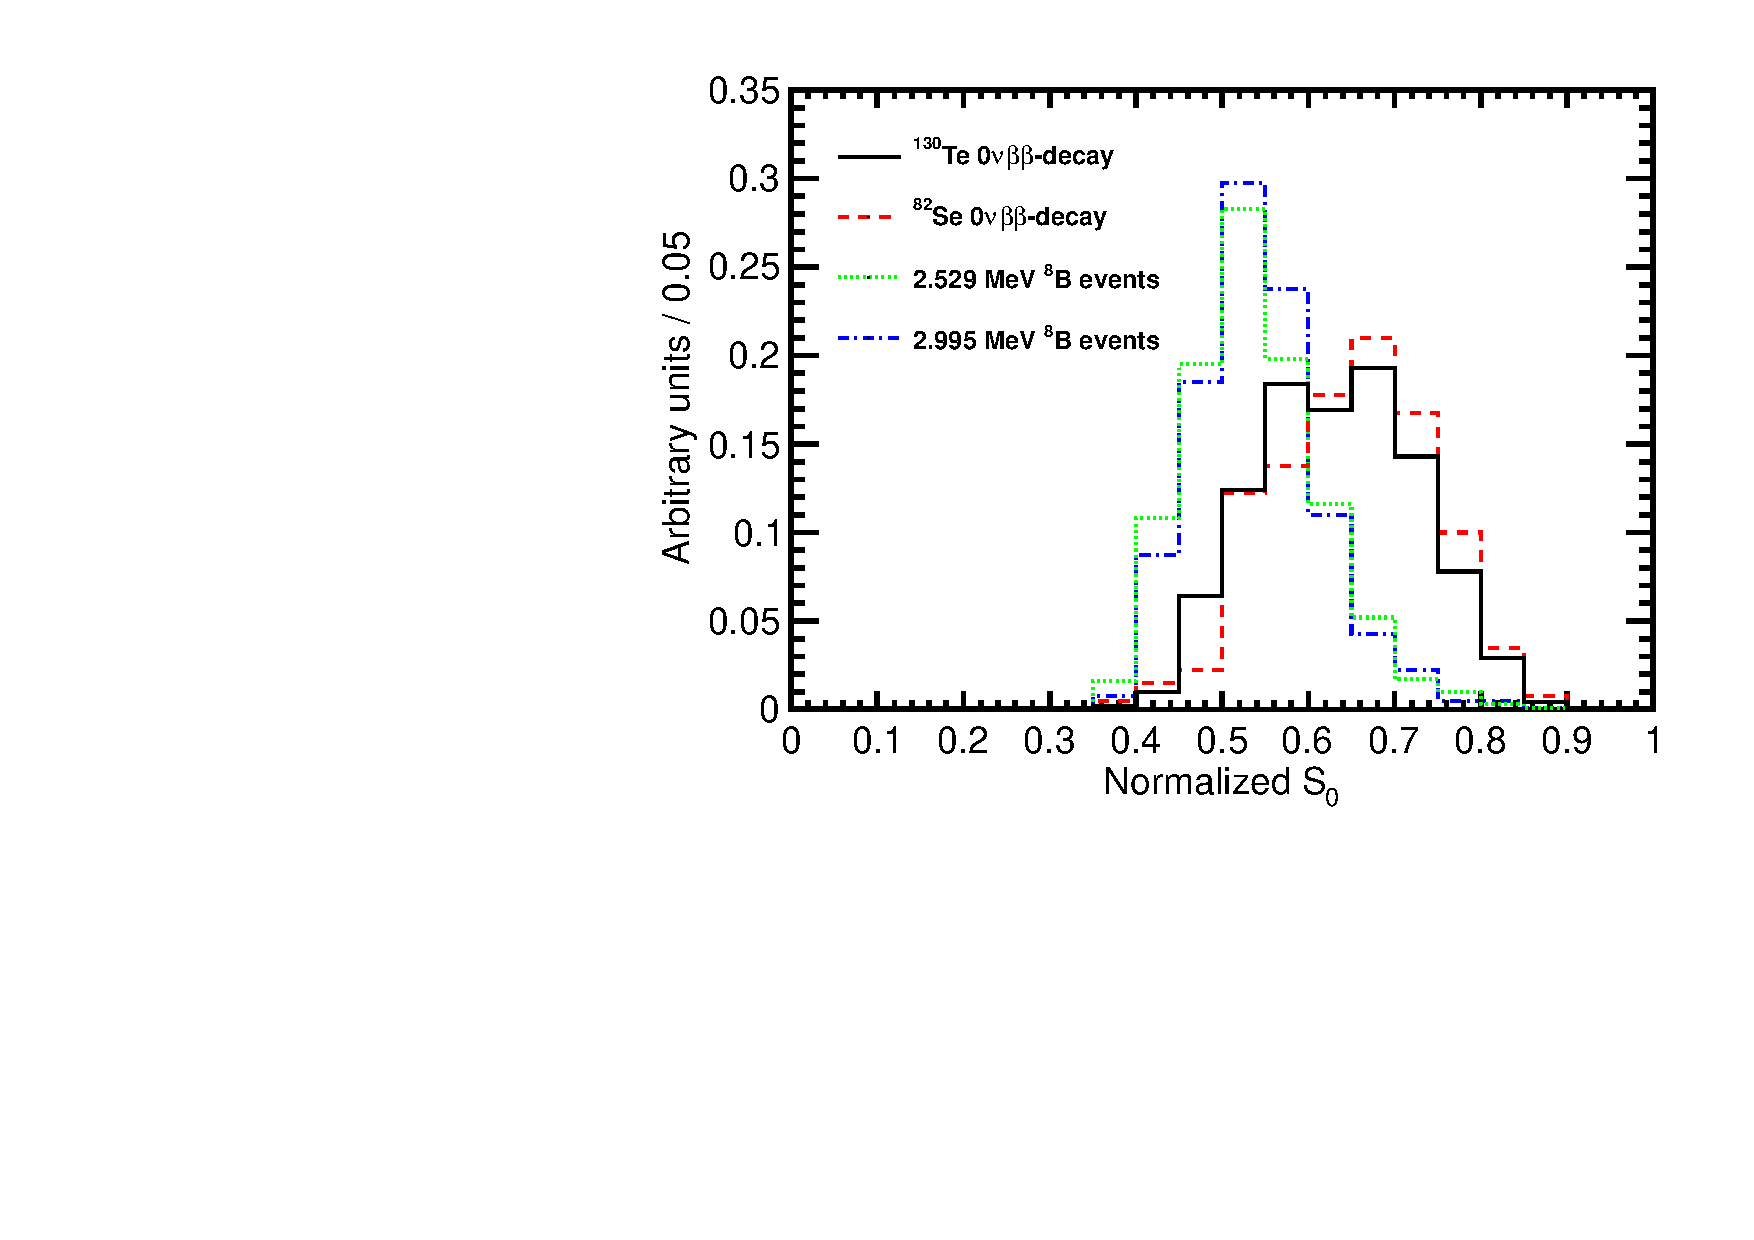
\includegraphics[angle=0,width=0.49\textwidth]{plots/hS0.pdf}
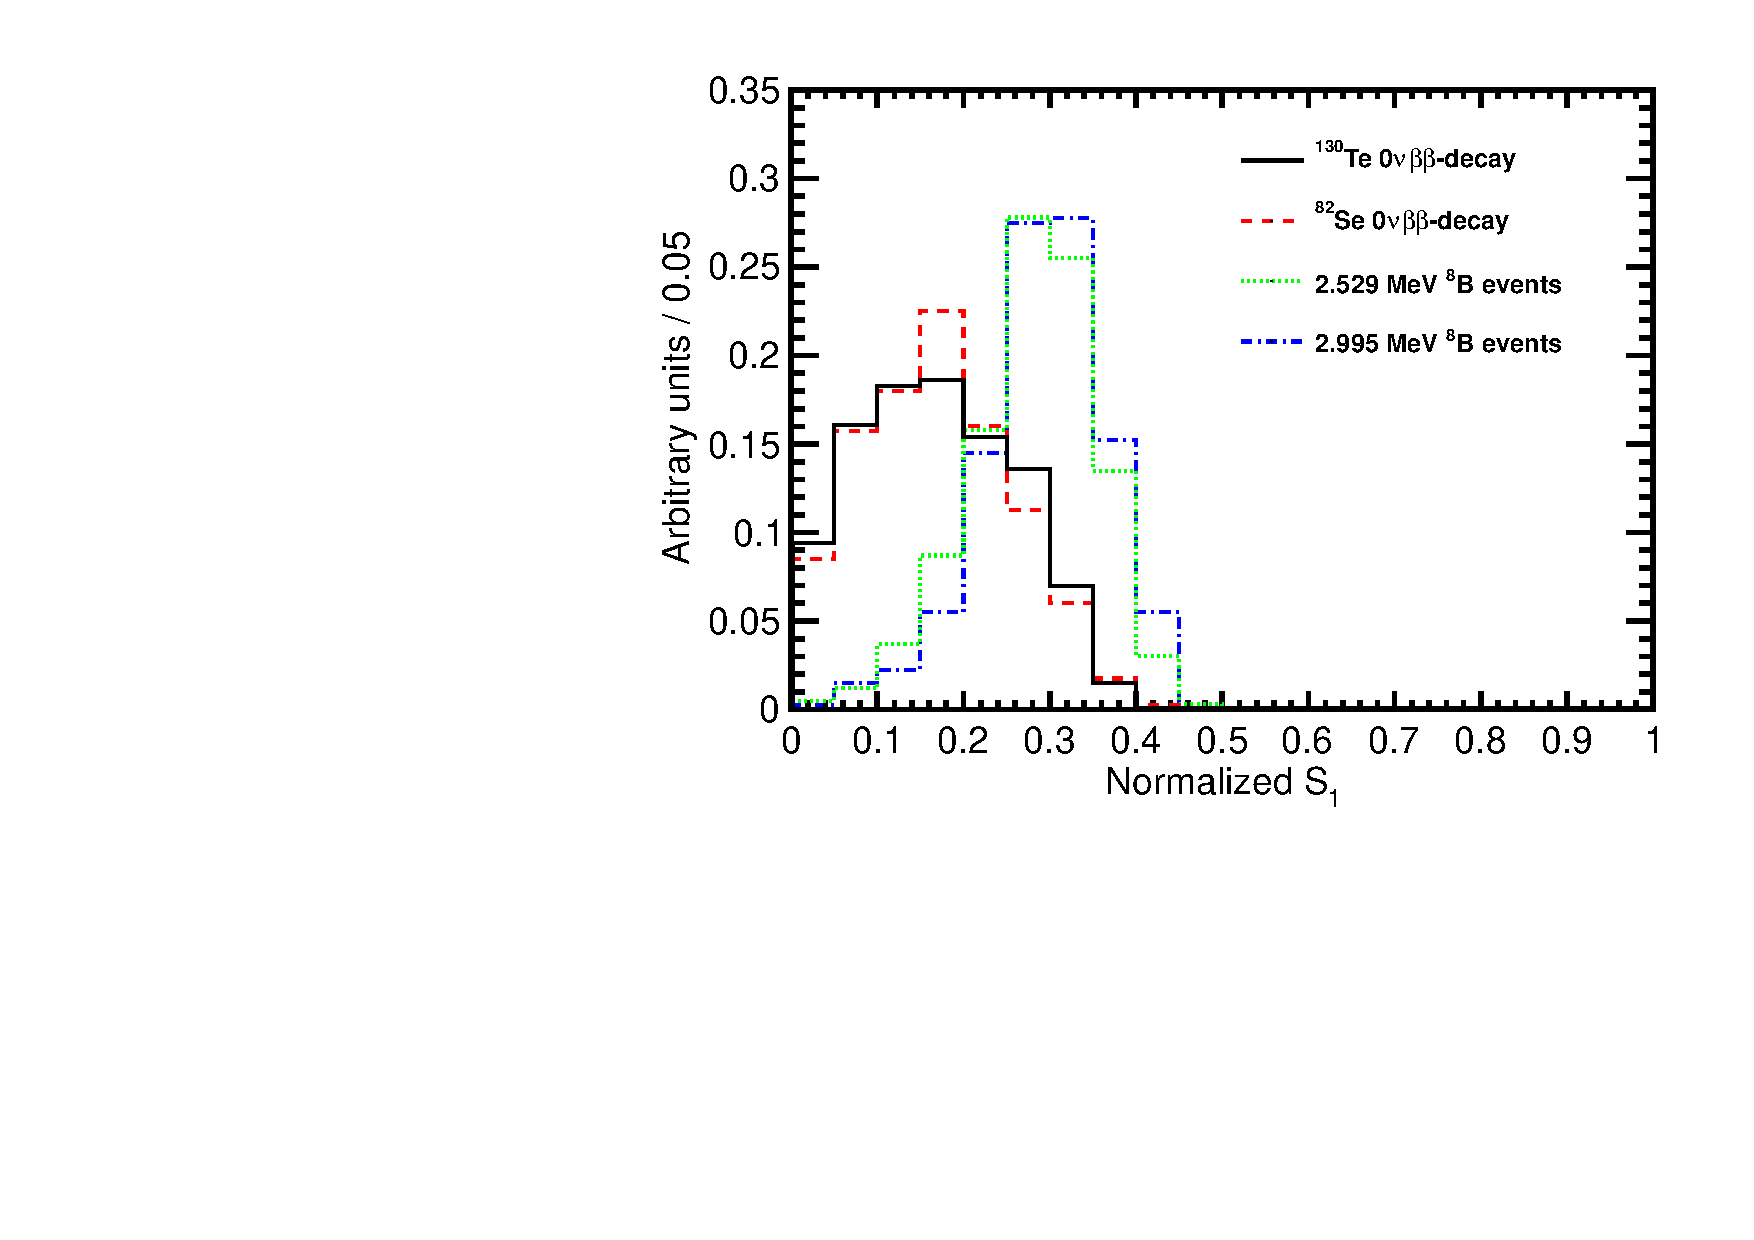
\includegraphics[angle=0,width=0.49\textwidth]{plots/hS1.pdf}
\caption{$S_0$ (left) and $S_1$ (right) distributions for events with two different event topologies and total kinetic energy. $^{130}Te$, $^{82}Se$ $\vbb$-decay, 2.529 MeV and 2.995 MeV events are compared. The simulation is done for events with the vertex in the center of the detector. $\B$ events are implemented as 2.529~MeV or 2.995~MeV electrons with initial direction along $x$-axis. Perfect vertex reconstruction - true vertex position is used. Time cut of 33.5~ns on the photon arrival time is applied.}
\label{fig:S_vs_energy}
\end{figure}


Figure~\ref{fig:SL_Te_33p5ns_center} shows separation between $\Te$ signal and $\B$ background events simulated at the center of the detector. True values of vertex position and time is used. Time cut of 33.5~ns on the photon arrival time is applied to separate Cherenkov and scintillation light. Most of the discrimination between signal and background comes from $S_0$ and $S_1$. In the following $S_2$ and $S_3$ are not used to separate $\Te$ and $\B$ events\footnote{$S_2$ and $S_3$ are helpful for separation of $\Te$ signal from $\Cten$ background. See Appendix.}. The scatter plot of $S_2$ vs $S_3$ is shown here for completeness. 

In order to optimize separation between $\Te$ signal and $\B$ background a linear combination of $S_0$ and $S_1$, $S_{01}$, is used. A linear fit, $S_0$ = $A \times S_1 + B$, of 2-dimensional $S_0$ vs $S_1$ scatter plot is performed as shown in Fig.~\ref{fig:SL_Te_33p5ns_center}. Then this 2-dimensional distribution is projected onto the fitted line. {\bf A little bit of math here to quantitatively describe $S_{01}$ via $S_0$ and $S_1$:} A new coordinate frame is obtained by rotation of the original $S_0$-$S_1$ frame at angle $\theta$ obtained from the fit: $tan(\theta)$=$A$. A transformation, $S_{01} = S_1 \cdot cos(\theta) + S_0 \cdot sin(\theta)$, defines the $S_{01}$ variable.

Bottom plot in Fig.~\ref{fig:SL_Te_33p5ns_center} shows performance of the $S_{01}$ variable to separate $\Te$ signal and $\B$ background. A fit to this distribution can be done to optimize the discrimination power in a particular experimental settings. Here we refrain from quantitative estimates on the improvements in sensitivity to $\vbb$-decay search using this method of spherical harmonics as a reliable estimate would require a dedicated analysis taking into account all the details of a particular experiment.

\begin{figure}[htb]
\centering
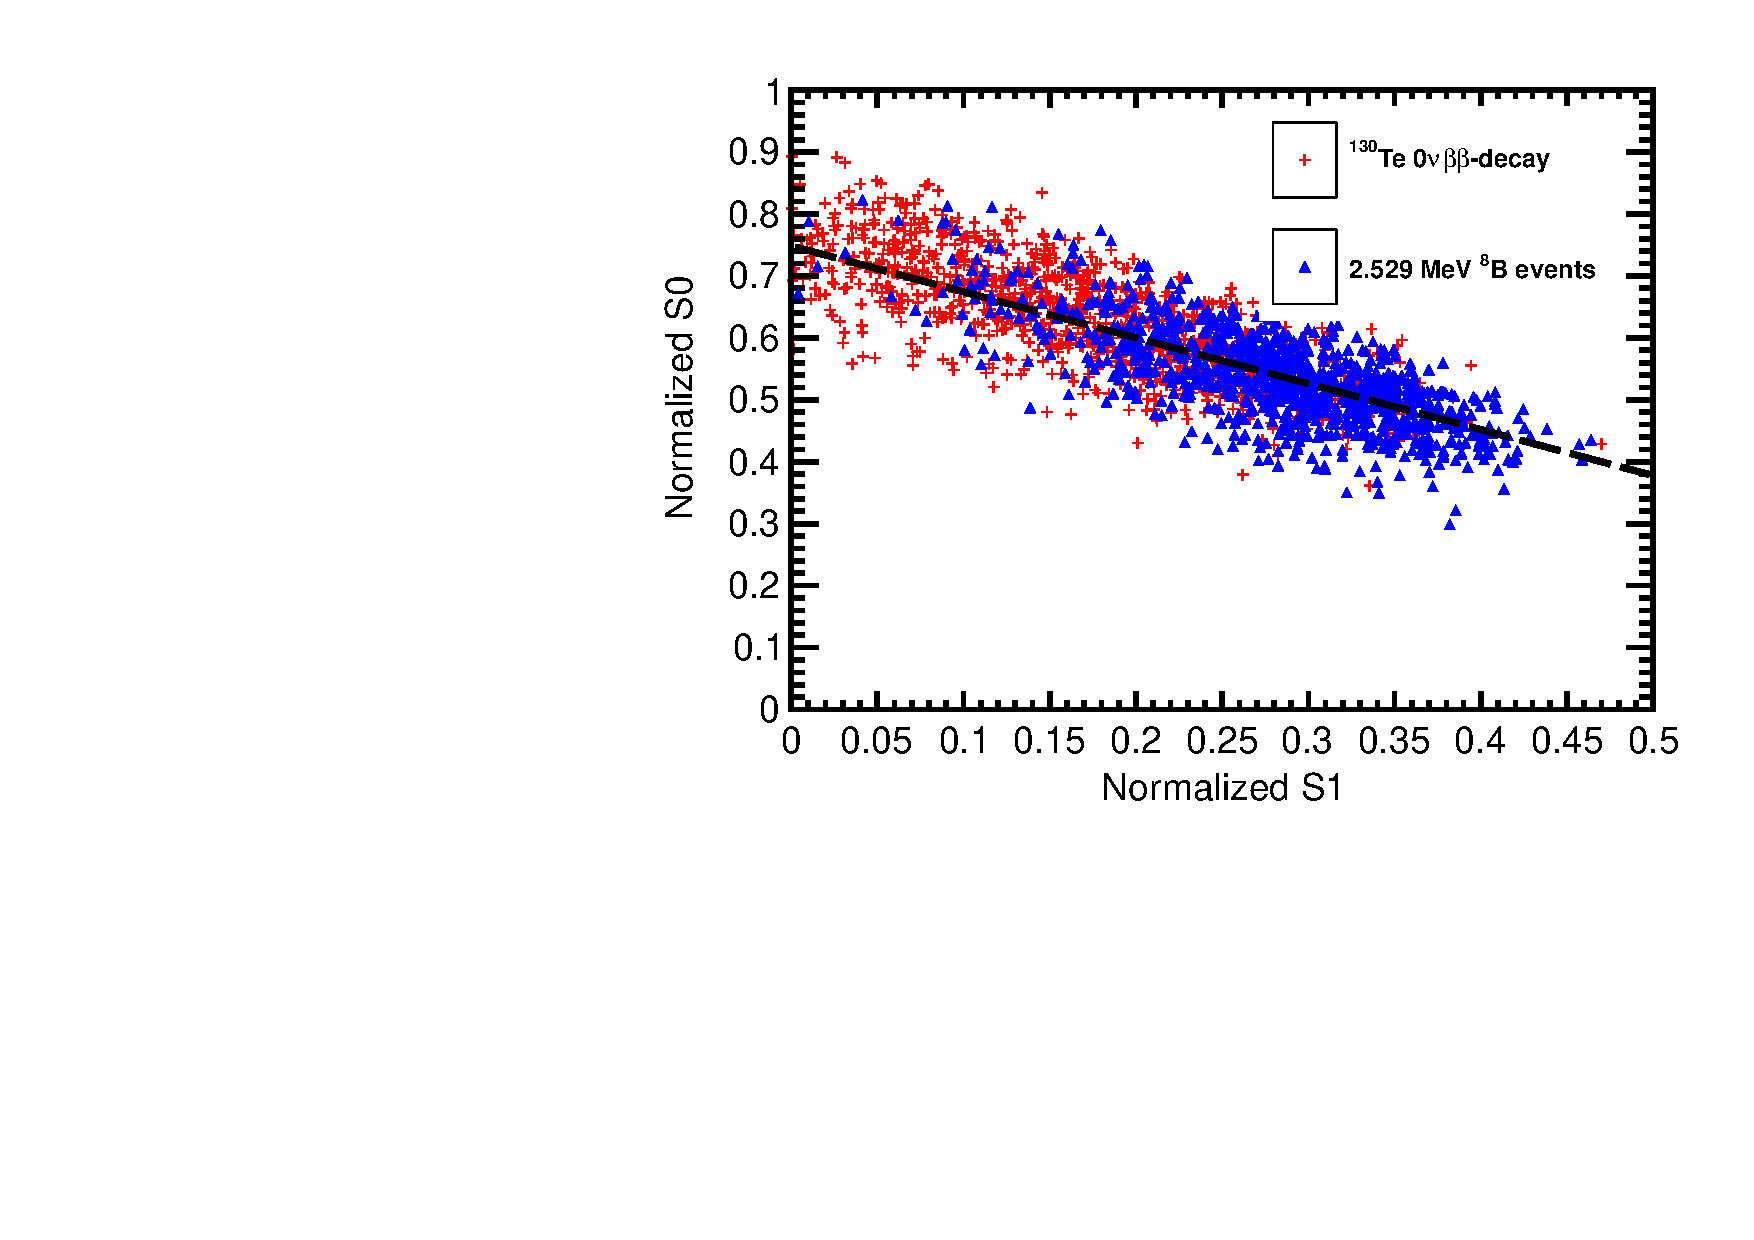
\includegraphics[angle=0,width=0.49\textwidth]{plots/hS0vsS1_Te130_1el_allLight_VtxSmear0cm_VtxShiftX0cm_33p5ns_center.pdf}
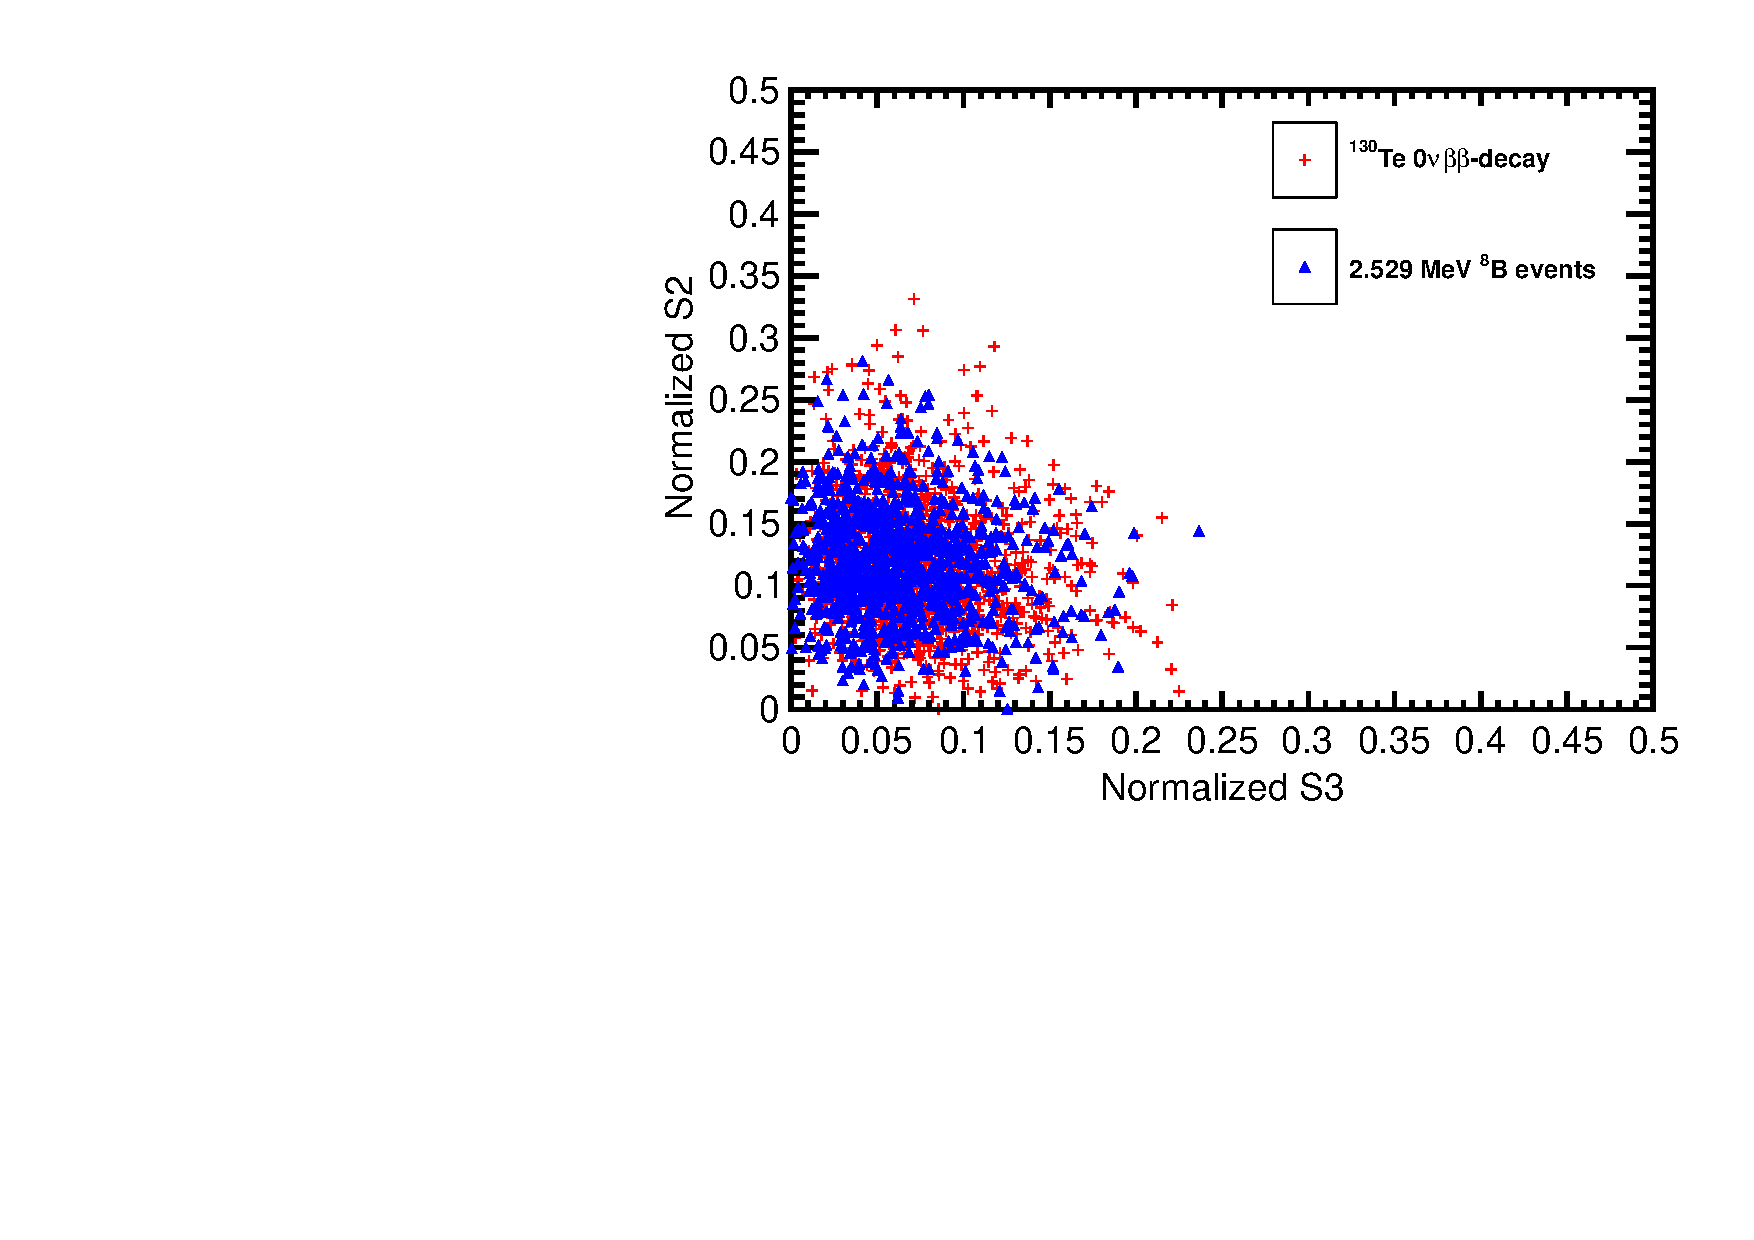
\includegraphics[angle=0,width=0.49\textwidth]{plots/hS2vsS3_Te130_1el_allLight_VtxSmear0cm_VtxShiftX0cm_33p5ns_center.pdf}
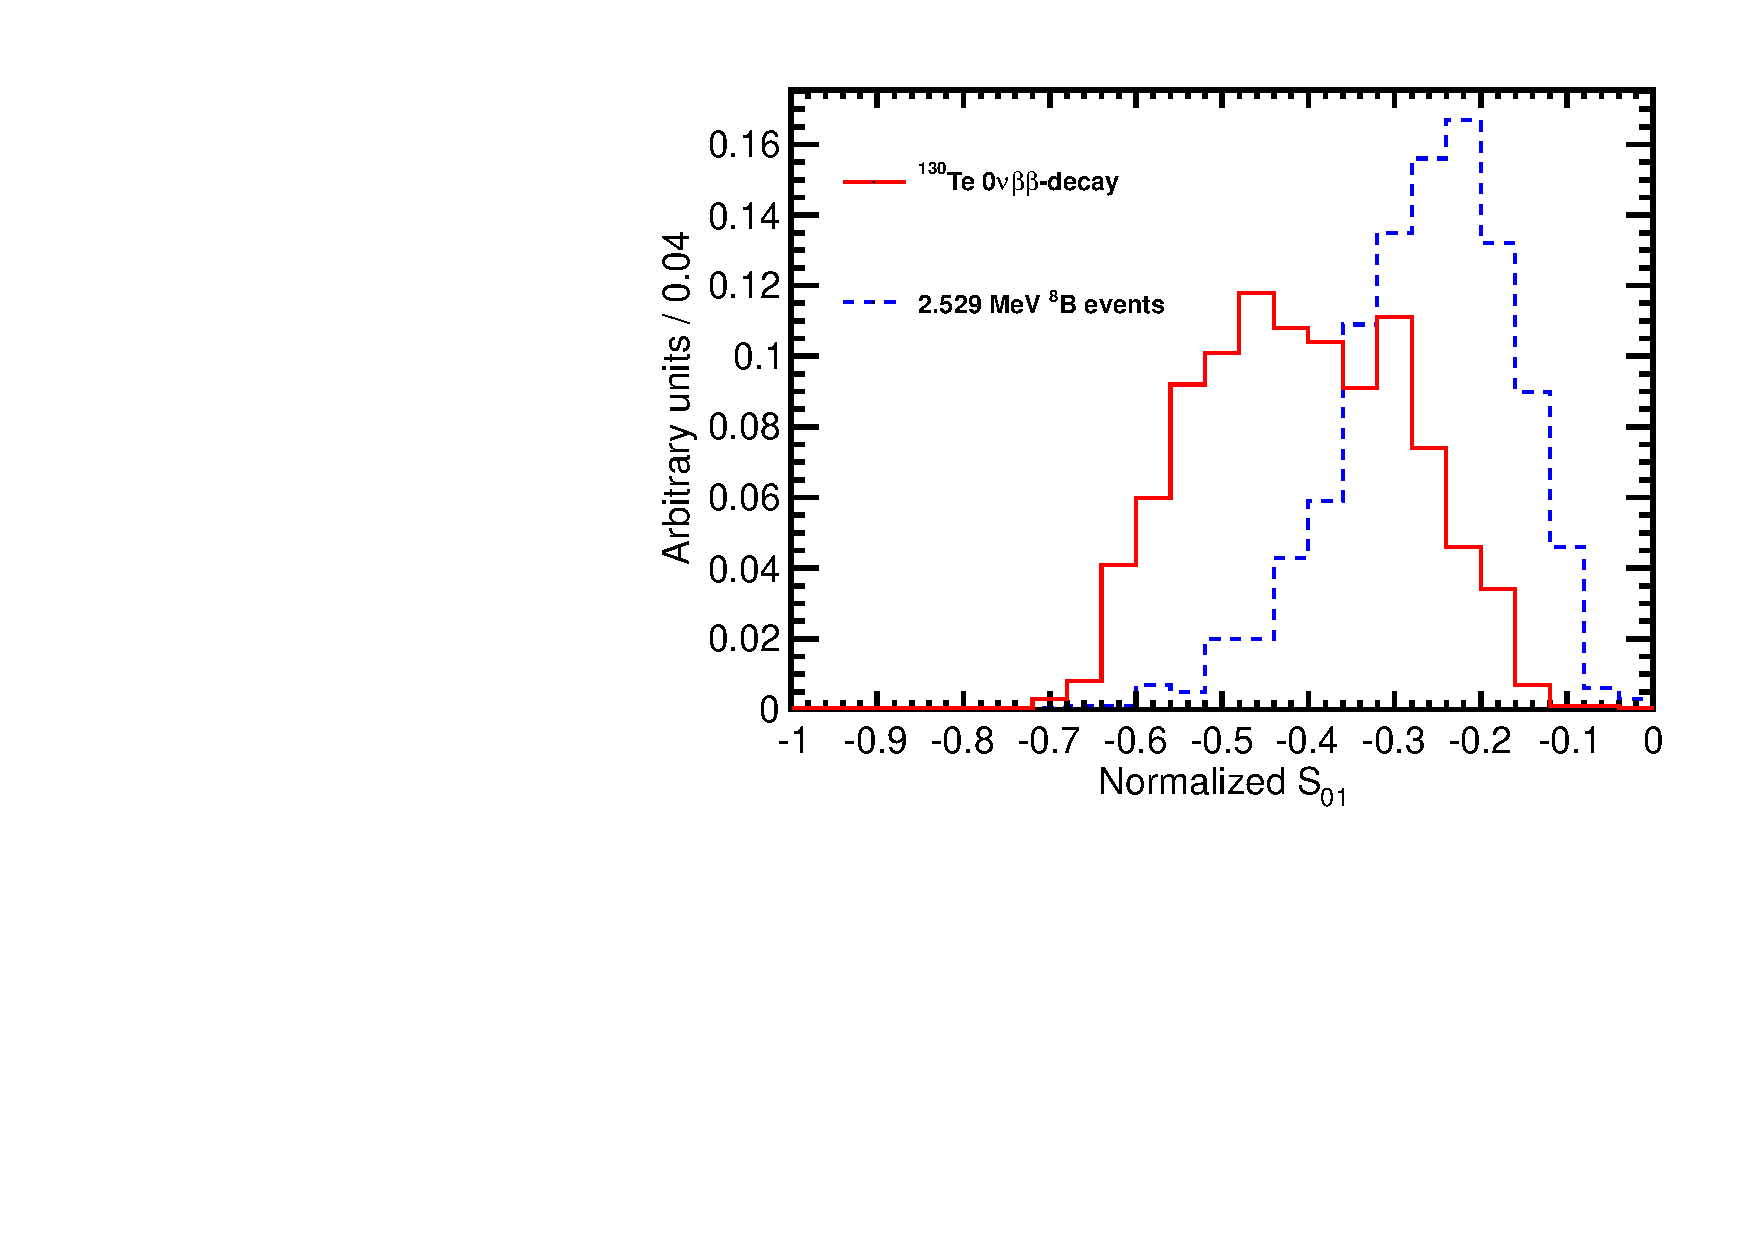
\includegraphics[angle=0,width=0.9\textwidth]{plots/hS01_allLight_VtxSmear0cm_VtxShiftX0cm_33p5ns_center.pdf}
\caption{Spherical harmonics comparison between $\Te$ $\vbb$-decay signal (Q$=$2.529~MeV) (red) and $\B$ solar neutrinos background (blue) for 1000 simulated events originated at the center of the sphere. $\B$ events are implemented as 2.529~MeV electrons with initial direction along $x$-axis. Perfect vertex reconstruction - true vertex position is used. Time cut of 33.5~ns on the photon arrival time is applied. (Top left) S$_0$ versus S$_1$ scatter plot. Black dotted line is a linear fit of these 2D histograms. Variable S$_{01}$ is defined as a projection of 2D distribution onto this linear fit. (Top right) S$_2$ versus S$_3$ scatter plot. (Bottom) $S_{01}$ distribution for the signal and background.}
\label{fig:SL_Te_33p5ns_center}
\end{figure}


\section{Experimental challenges}

So far only events at the center of the detector have been considered. In this section we discuss performance of the spherical harmonics analysis for events distributed within the fiducial volume of the detector taking into account finite resolution on vertex position reconstruction.

When the vertex is not at the center, a uniform time cut on the photon arrival time is no longer effective in the selection of Cherenkov photons. In the case of off-center vertex, even significantly delayed scintillation photons can reach the side of the detector that is closer to the vertex much earlier than Cherenkov photons traveling to the opposite side of the detector. Therefore, the time cut has to be position dependent and take into account the total distance traveled by each individual photon.

We found that the time cut defined as $\Delta t$=$t^{phot}_{measured} - t^{phot}_{predicted}$$<$1~ns selects photons with sufficient fraction of Cherenkov photons. Predicted time, $ t^{phot}_{predicted}$=$l/v^{phot}$, depends on total distance, $l$, traveled by the photon and proper assignment of the velocity for each photon, $v^{phot}$, that depends on index of refraction\footnote{We use average index of refraction of n=1.53}. Therefore the relative Cherenkov/scintillation composition of the light selected with this $\Delta t$ time cut depends on the vertex location and chromatic dispersions. 

Due to chromatic dispersion, even with perfect vertex reconstruction one cannot achieve the same level of separation between Chrerenkov and scintillation light compared to the central events considered above in Section 4. This in turn reduces the effectiveness of the spherical harmonics analysis in separating of $\vbb$-decay and $\B$ events (see Fig.~\ref{fig:SL_Te_SmearX0cm_momDT1ns_rndVtx_3p0m}). However next generation detectors can recover losses due to chromatic dispersion by choosing liquid scintillators with a more narrow emission spectrum.


\begin{figure}[htb]
\centering
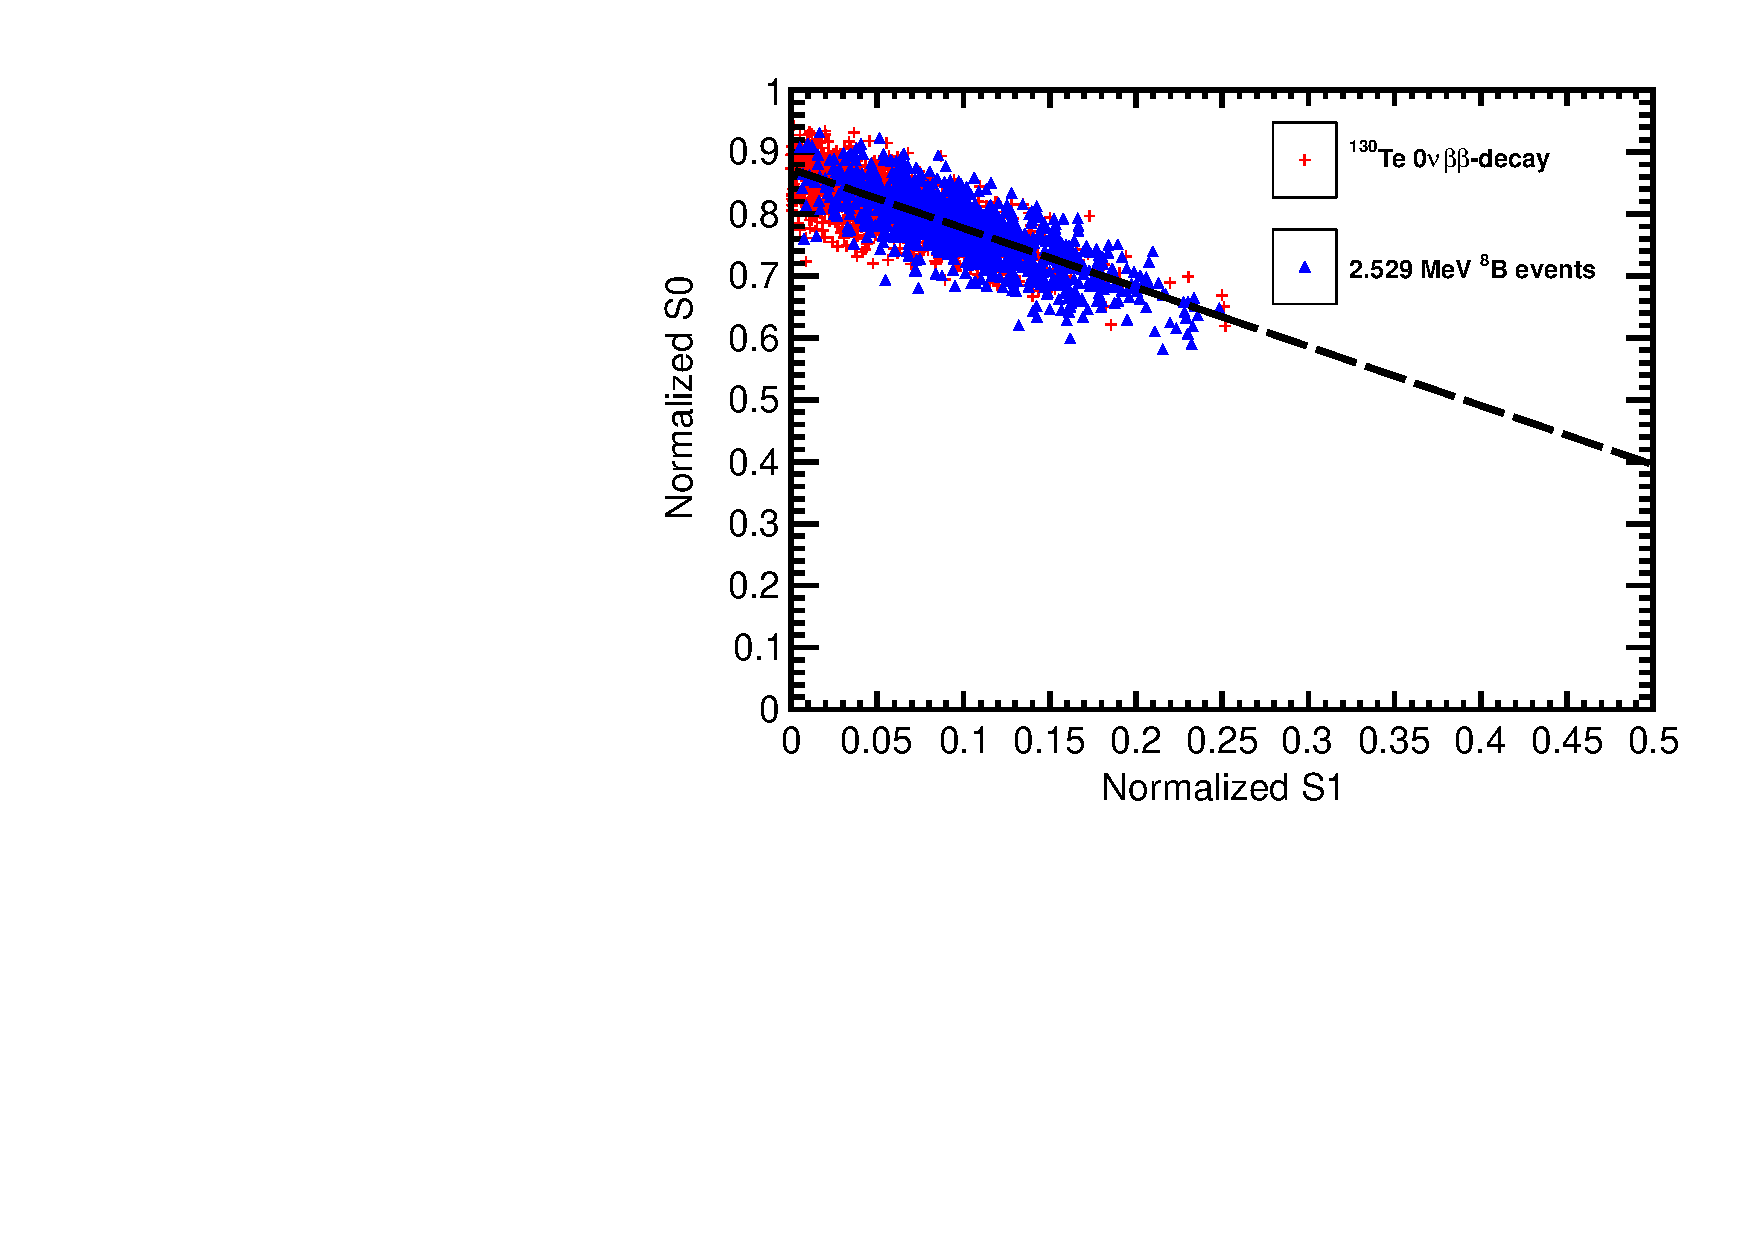
\includegraphics[angle=0,width=0.49\textwidth]{plots/hS0vsS1_Te130_1el_allLight_VtxSmear0cm_VtxShiftX0cm_momDT1p0ns_rndVtx_3p0mSphere.pdf}
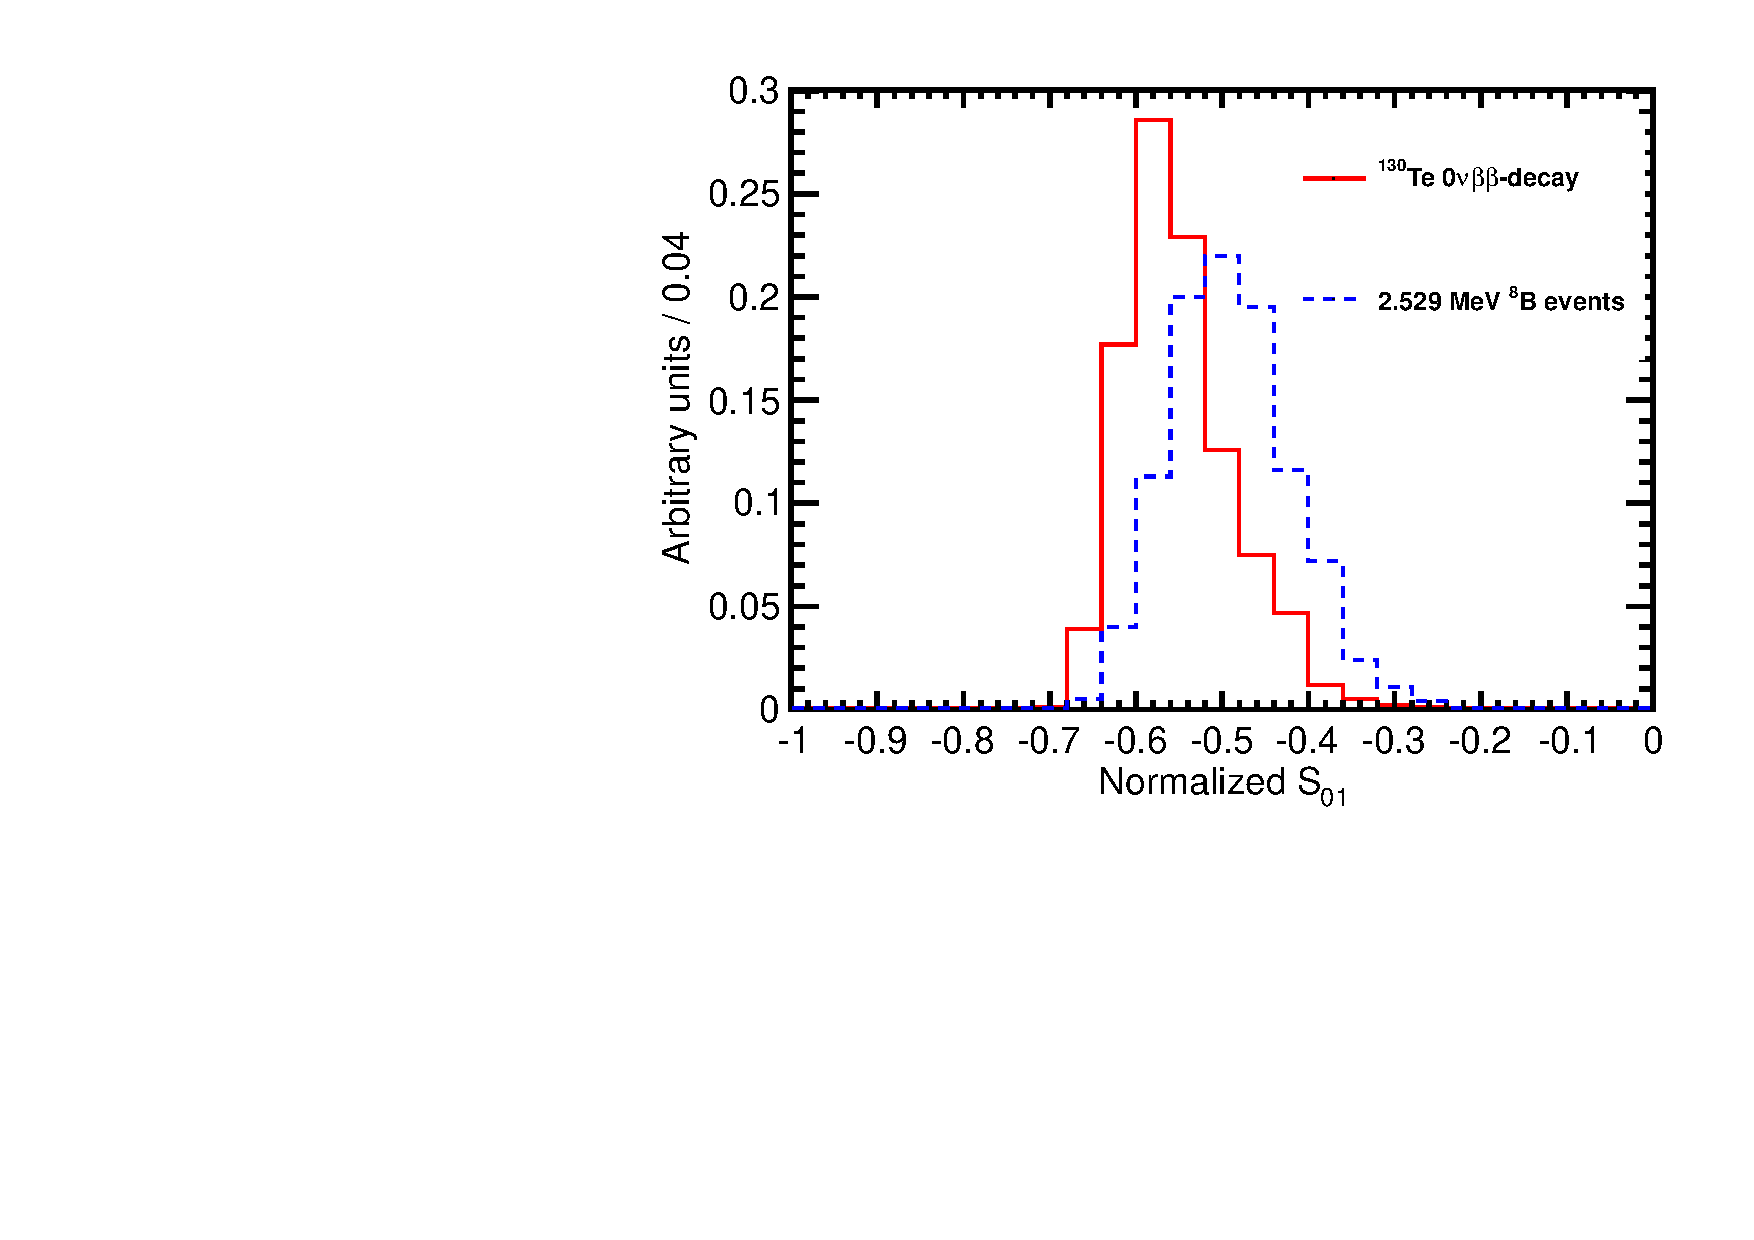
\includegraphics[angle=0,width=0.49\textwidth]{plots/hS01_allLight_VtxSmear0cm_VtxShiftX0cm_momDT1p0ns_rndVtx_3p0mSphere.pdf}
\caption{Spherical harmonics comparison between $\Te$ $\vbb$-decay signal (Q$=$2.529~MeV) (red) and $\B$ solar neutrinos background (blue) for 1000 simulated events.Verticies are uniformly distributed within the fiducial volume, R$<$3~m. $^8$Be events are implemented as 2.529~MeV electrons with the initial momentum direction uniformly distributed within 4$\pi$ solid angle. Perfect vertex reconstruction - true vertex position is used. (Left) S$_0$ versus S$_1$ scatter plot. Black dotted line is a linear fit of these 2D histograms. Variable S$_{01}$ is defined as a projection of 2D distribution onto this linear fit. (Right) S$_{01}$}
\label{fig:SL_Te_SmearX0cm_momDT1ns_rndVtx_3p0m}
\end{figure}



Imprecise knowledge of the vertex position due to finite resolution is another factor affecting performance of the spherical harmonics analysis. Small deviations in vertex reconstruction cause large effect on $S_0$ and $S_1$ for single electron event topology. For the verticies shifted along the direction of the electron the $\Delta t$ cut makes uniform scintillation light distribution less uniform. The $\Delta t$ cut selects more forward emitted photons in the case when the reconstructed vertex is shifted to the direction opposite to the electron momentum (enhancing forward region populated by Cherenkov photons - more asymmetric photon distribution causing higher values of $S_1$). It selects more backward emitted photons in the case when the reconstructed vertex is shifted in the direction along the electron momentum (counter balancing forward region populated by Cherenkov photons - more symmetric photon distribution causing smaller values of $S_1$).

\begin{figure}[htb]
\centering
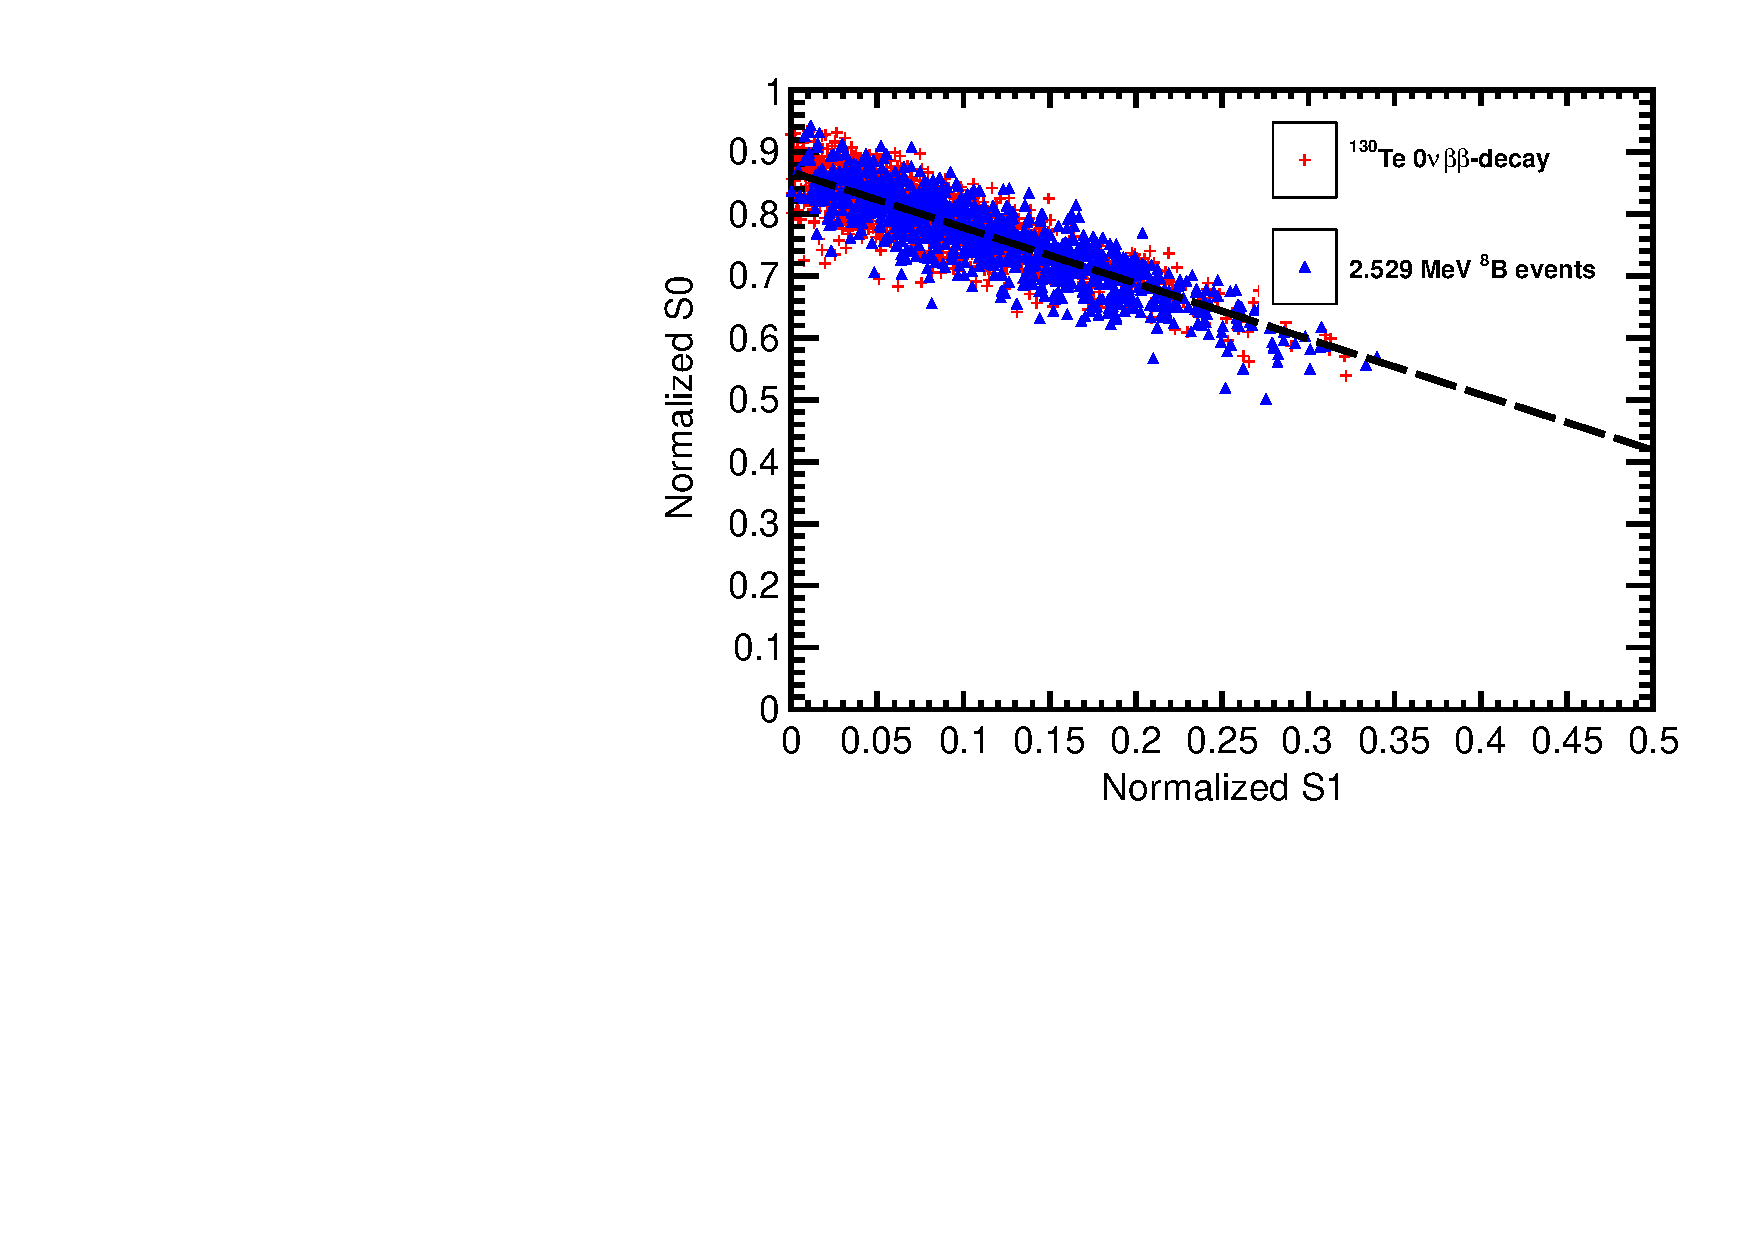
\includegraphics[angle=0,width=0.49\textwidth]{plots/hS0vsS1_Te130_1el_allLight_VtxSmear3cm_VtxShiftX0cm_momDT1p0ns_rndVtx_3p0mSphere.pdf}
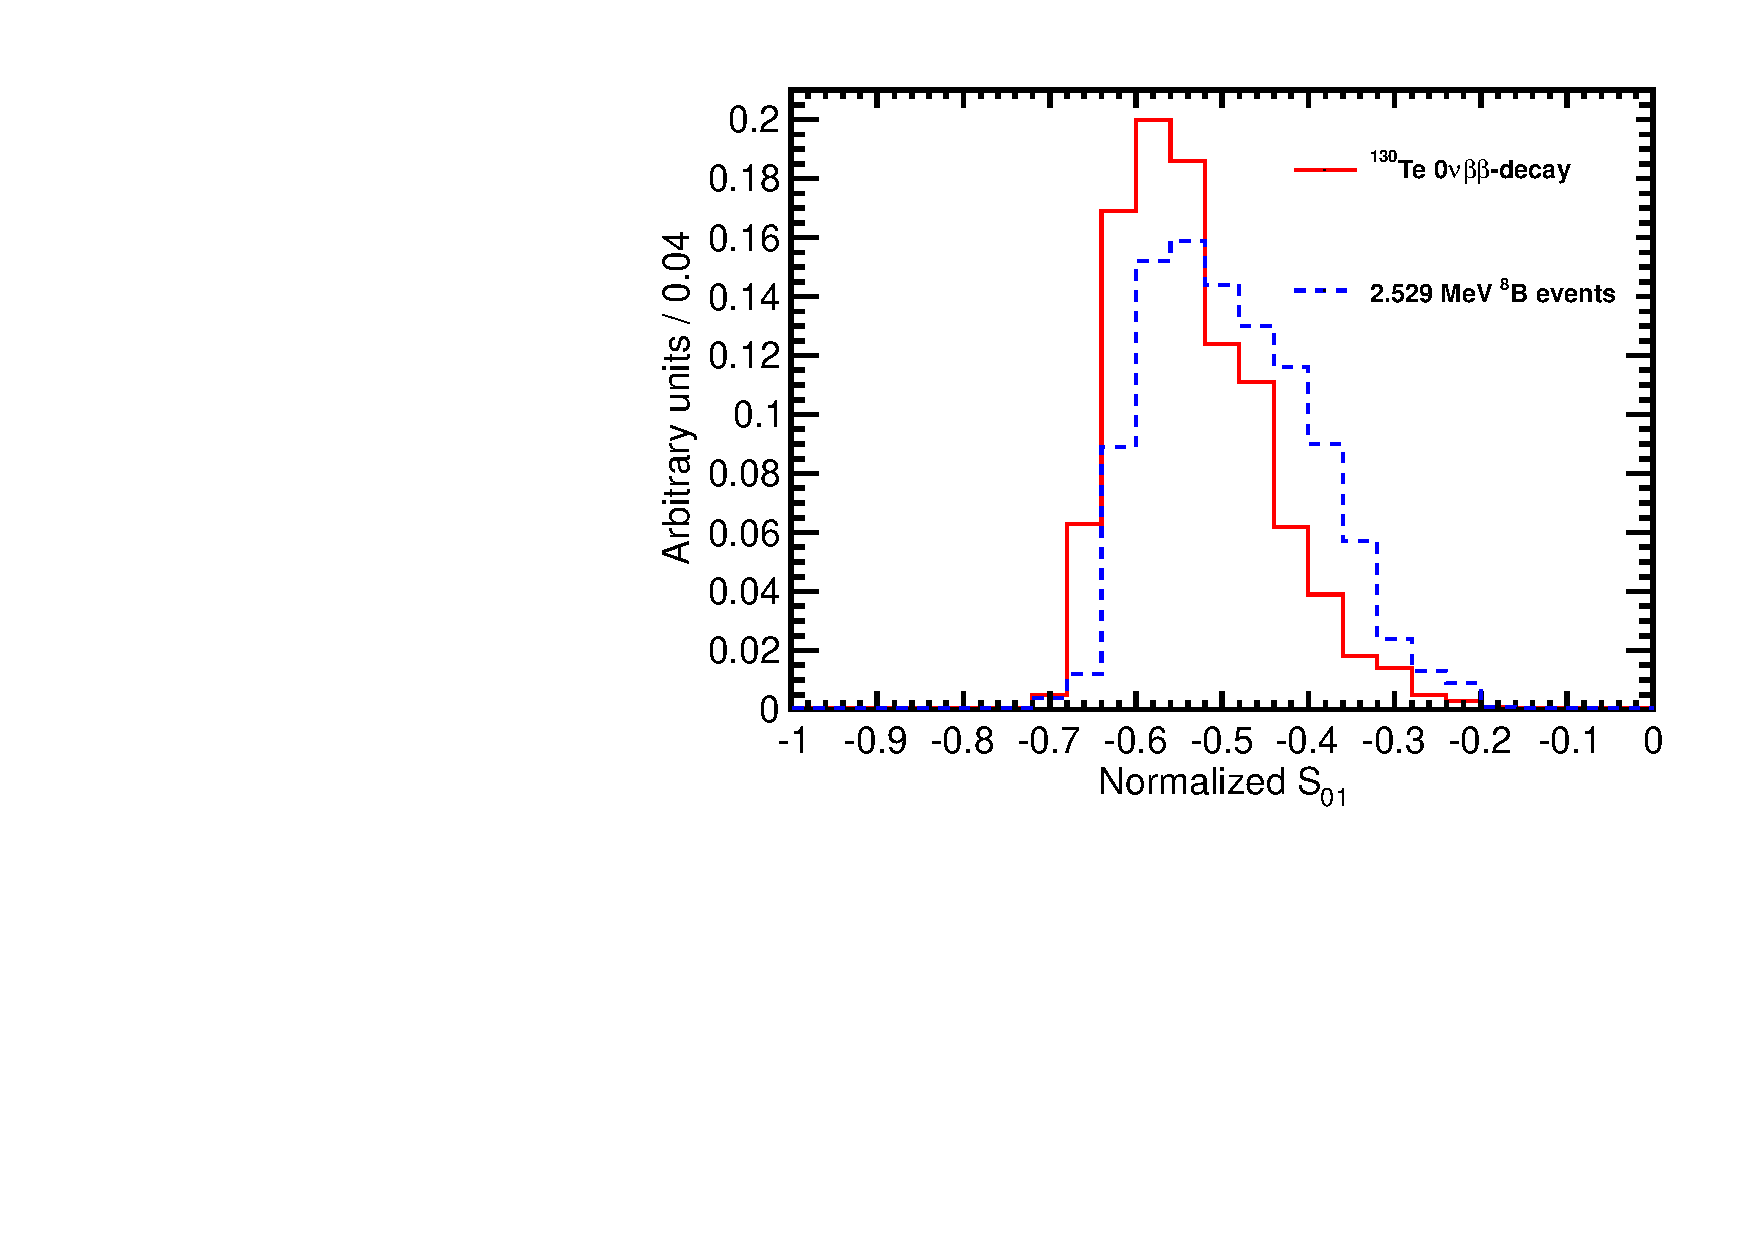
\includegraphics[angle=0,width=0.49\textwidth]{plots/hS01_allLight_VtxSmear3cm_VtxShiftX0cm_momDT1p0ns_rndVtx_3p0mSphere.pdf}
\caption{Spherical harmonics comparison between $\Te$ $\vbb$-decay signal (Q$=$2.529~MeV) (red) and $\B$ solar neutrinos background (blue) for 1000 simulated events.Verticies are uniformly distributed within the fiducial volume, R$<$3~m. $^8$Be events are implemented as 2.529~MeV electrons with the initial momentum direction uniformly distributed within 4$\pi$ solid angle. Vetrex is smeared with 3~cm resolution. (Left) S$_0$ versus S$_1$ scatter plot. Black dotted line is a linear fit of these 2D histograms. Variable S$_{01}$ is defined as a projection of 2D distribution onto this linear fit. (Right) S$_{01}$}
\label{fig:SL_Te_SmearX3cm_momDT1ns_rndVtx_3p0m}
\end{figure}


{\bf Solution to this problem would be a better selection criteria of early light. It has to preserve high admixture of the Cherenkov photons, but needs to select scintillation photons in a more uniform manner. Working on it, but may not be simple so I don't want to include it in this paper.}

Good vertex resolution is essential for spherical harmonics analysis. Such strong dependence on the vertex resolution can be addressed by choosing a different liquid scintillator mixture with a more delayed emission of the scintillation  light. Figure~\ref{fig:SL_Te_momDT1ns_sci0p5ns_rndVtx_3p0m} shows spherical harmonics calculated for the time profile which has scintillation component delayed by 0.5ns with respect to what is shown in Fig.~\ref{fig:Arrival_time}


\begin{figure}[htb]
\centering
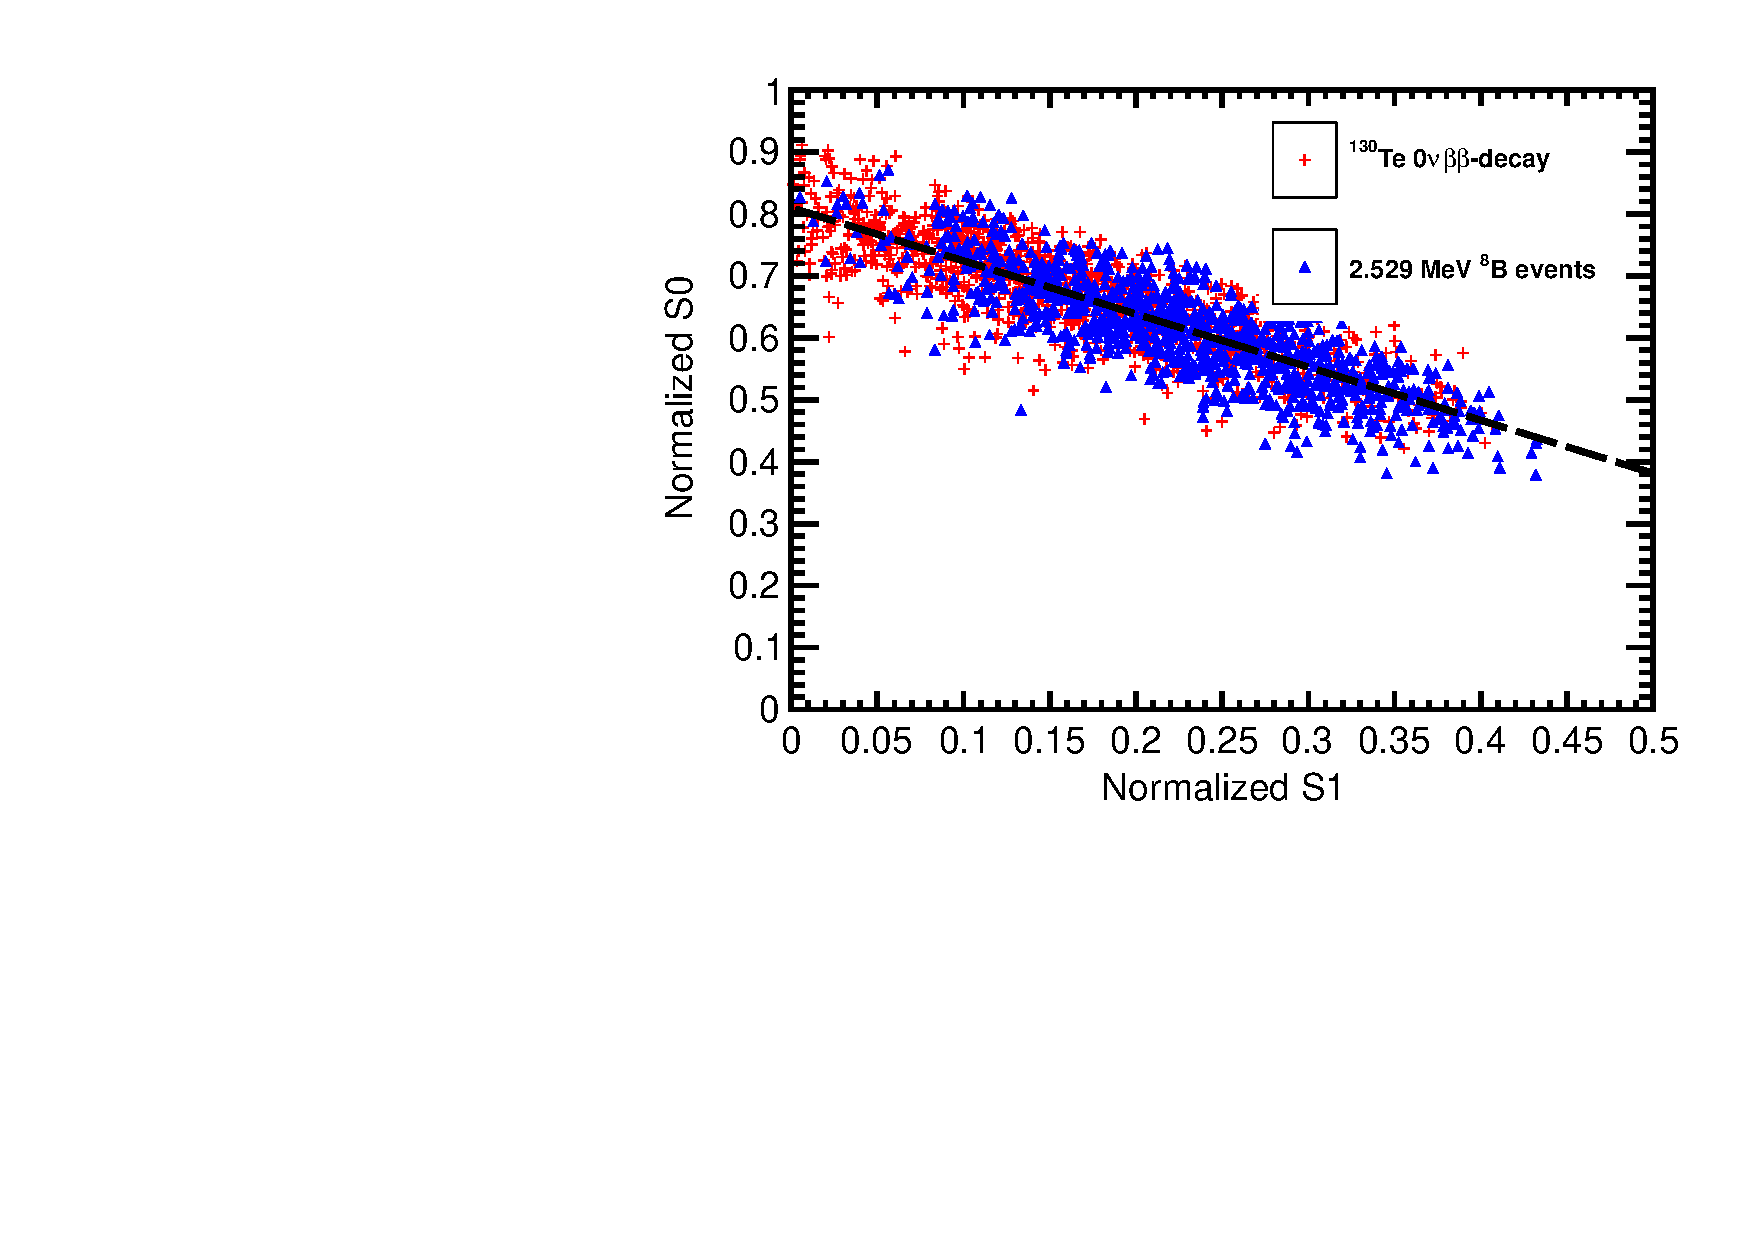
\includegraphics[angle=0,width=0.49\textwidth]{plots/hS0vsS1_Te130_1el_allLight_VtxSmear3cm_VtxShiftX0cm_momDT1p0ns_sci0p5ns_rndVtx_3p0mSphere.pdf}
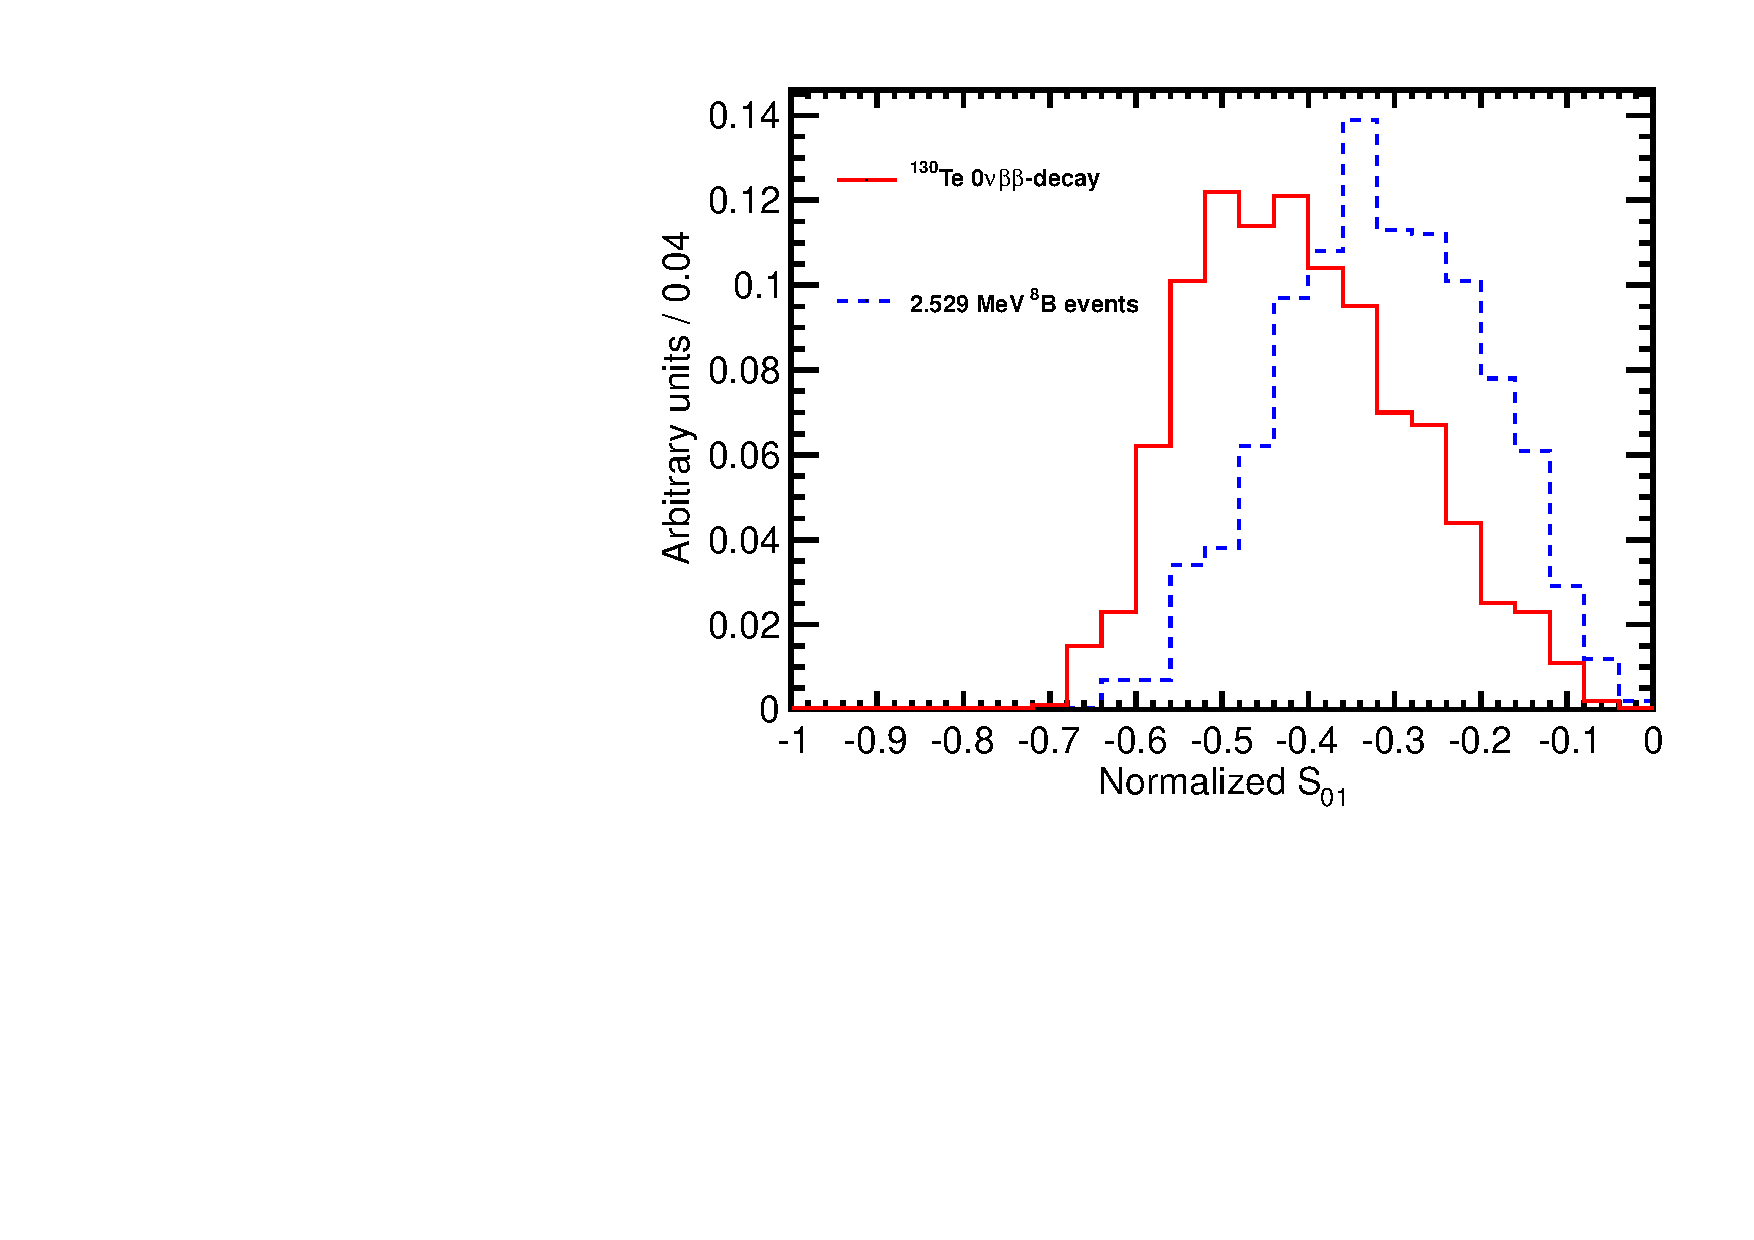
\includegraphics[angle=0,width=0.49\textwidth]{plots/hS01_allLight_VtxSmear3cm_VtxShiftX0cm_momDT1p0ns_sci0p5ns_rndVtx_3p0mSphere.pdf}
\caption{Spherical harmonics comparison between $\Te$ $\vbb$-decay signal (Q$=$2.529~MeV) (red) and $\B$ solar neutrinos background (blue) for 1000 simulated events.Verticies are uniformly distributed within the fiducial volume, R$<$3~m. $^8$Be events are implemented as 2.529~MeV electrons with the initial momentum direction uniformly distributed within 4$\pi$ solid angle. Vetrex is smeared with 3~cm resolution. {\bf Scintillation light is delayed by additional 0.5~ns.} (Left) S$_0$ versus S$_1$ scatter plot. Black dotted line is a linear fit of these 2D histograms. Variable S$_{01}$ is defined as a projection of 2D distribution onto this linear fit. (Right) S$_{01}$}
\label{fig:SL_Te_SmearX3cm_momDT1ns_sci0p5ns_rndVtx_3p0m}
\end{figure}


\section{Conclusions}
A technique based on spherical harmonics analysis is discussed to separate $\vbb$-decay from $\B$ solar neutrino interactions. The separation is based on distinct event topologies of signal and background. This event topology information is available in addition to the measurements of the energy deposited in the detector. This technique may be further developed and adopted by future large scale liquid scintillator detectors to suppress background coming from $\B$ solar neutrino interactions in the detector volume. The performance of the technique is mostly affected by chromatic dispersions, vertex reconstruction and time profile of the emission of the scintillation light. We show that a liquid scintillator detector with a $\sim$1~ns total delay of the scintillation light with respect to the Cherenkov light allows for use of spherical harmonics analysis as an extra handle to extract $\vbb$-decay signal.


\section{Acknowledgments}
To be finalized based on opt-in for the author list.
%We thank G.~Orebi-Gann for discussions on the backgrounds and sensitivity of the SNO+ experiment. We thankful to Evan Angelico for help with investigation of how various detector parameters affect vertex reconstruction. We thank Chandler Schlupf for help with sensitivity calculations. We thank Christopher Aberle, Brian Naranjo, Eric Spieglan and Matt Wetstein for fruitful discussions on event topology and vertex reconstruction. This work was done with support from DOE (grant number) and NSF (grant number).


\appendix

\section{$\vbb$-decay vs $^{10}$C background}

Other common backgrounds to $\vbb$-decay search include radioactive decays of nuclei excited by cosmic muons and decays of Th and U naturally present in the materials. In a liquid scintillator detectors most of events from Th and U decays are happening in the materials of the scintillator enclosure. Typically they enter the fiducial volume as 2.6~MeV gammas. These gammas either shower too late or have mis-reconstructed vertex. Both effects depend on details of a particular experiment and therefore in this paper we make no attempt to introduce a topology reconstruction for the backgrounds coming from Th and U lines. Cosmic induced backgrounds, to the contrary, are more generic and originate inside the fiducial volume. In this section we discuss event topology of $\Cten$ events that are most relevant in the energy of 2-3~MeV.

Typical energy deposition by $\Cten$ events is shown in Fig.~\ref{fig:Edep_C10}. We propose to use spherical harmonics analysis to separate $\vbb$-decay events from $\Cten$ events that within energy resolution overlap with the $\vbb$-decay Q-value.



\begin{figure}[htb]
\centering
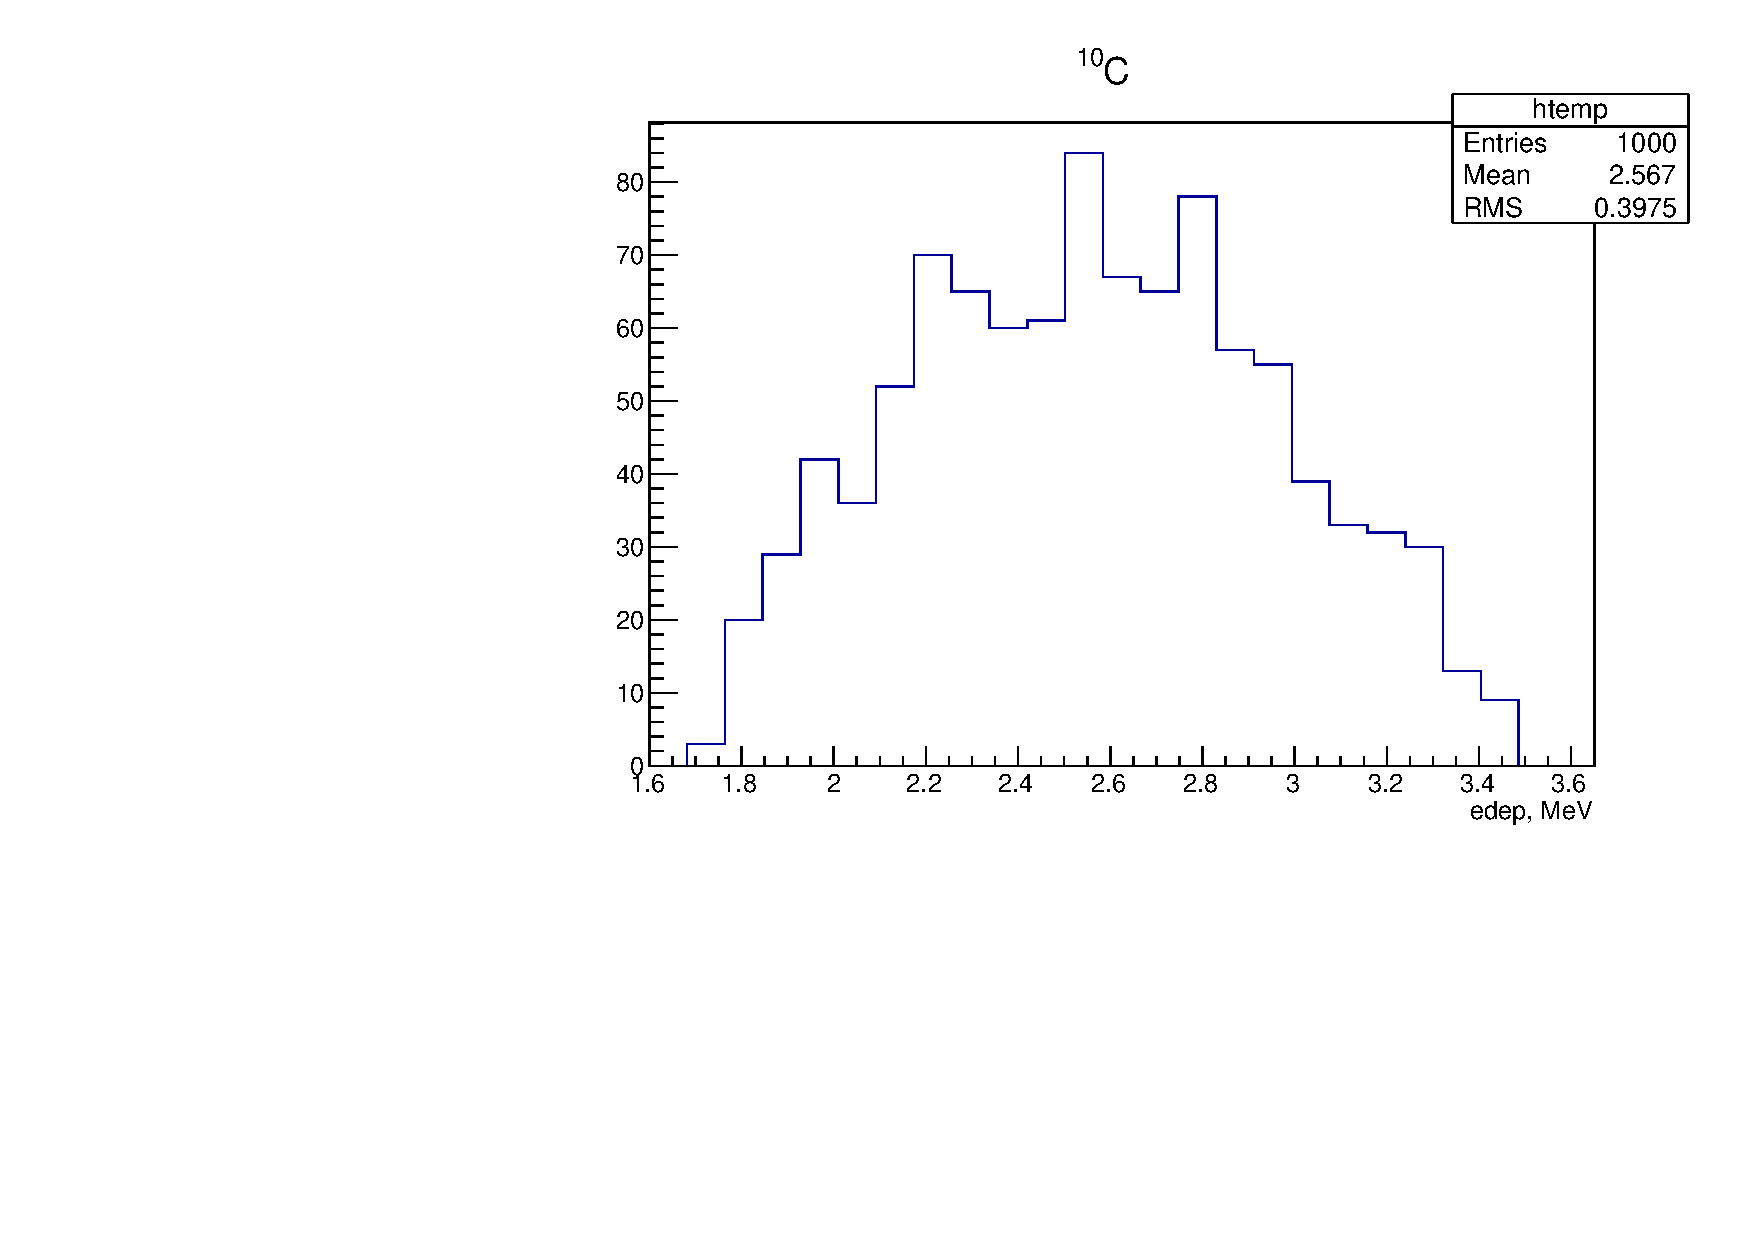
\includegraphics[angle=0,width=0.95\textwidth]{plots/hEdep_C10.pdf}
\caption{Energy deposition in $\Cten$ events.}
\label{fig:Edep_C10}
\end{figure}

\begin{figure}[htb]
\centering
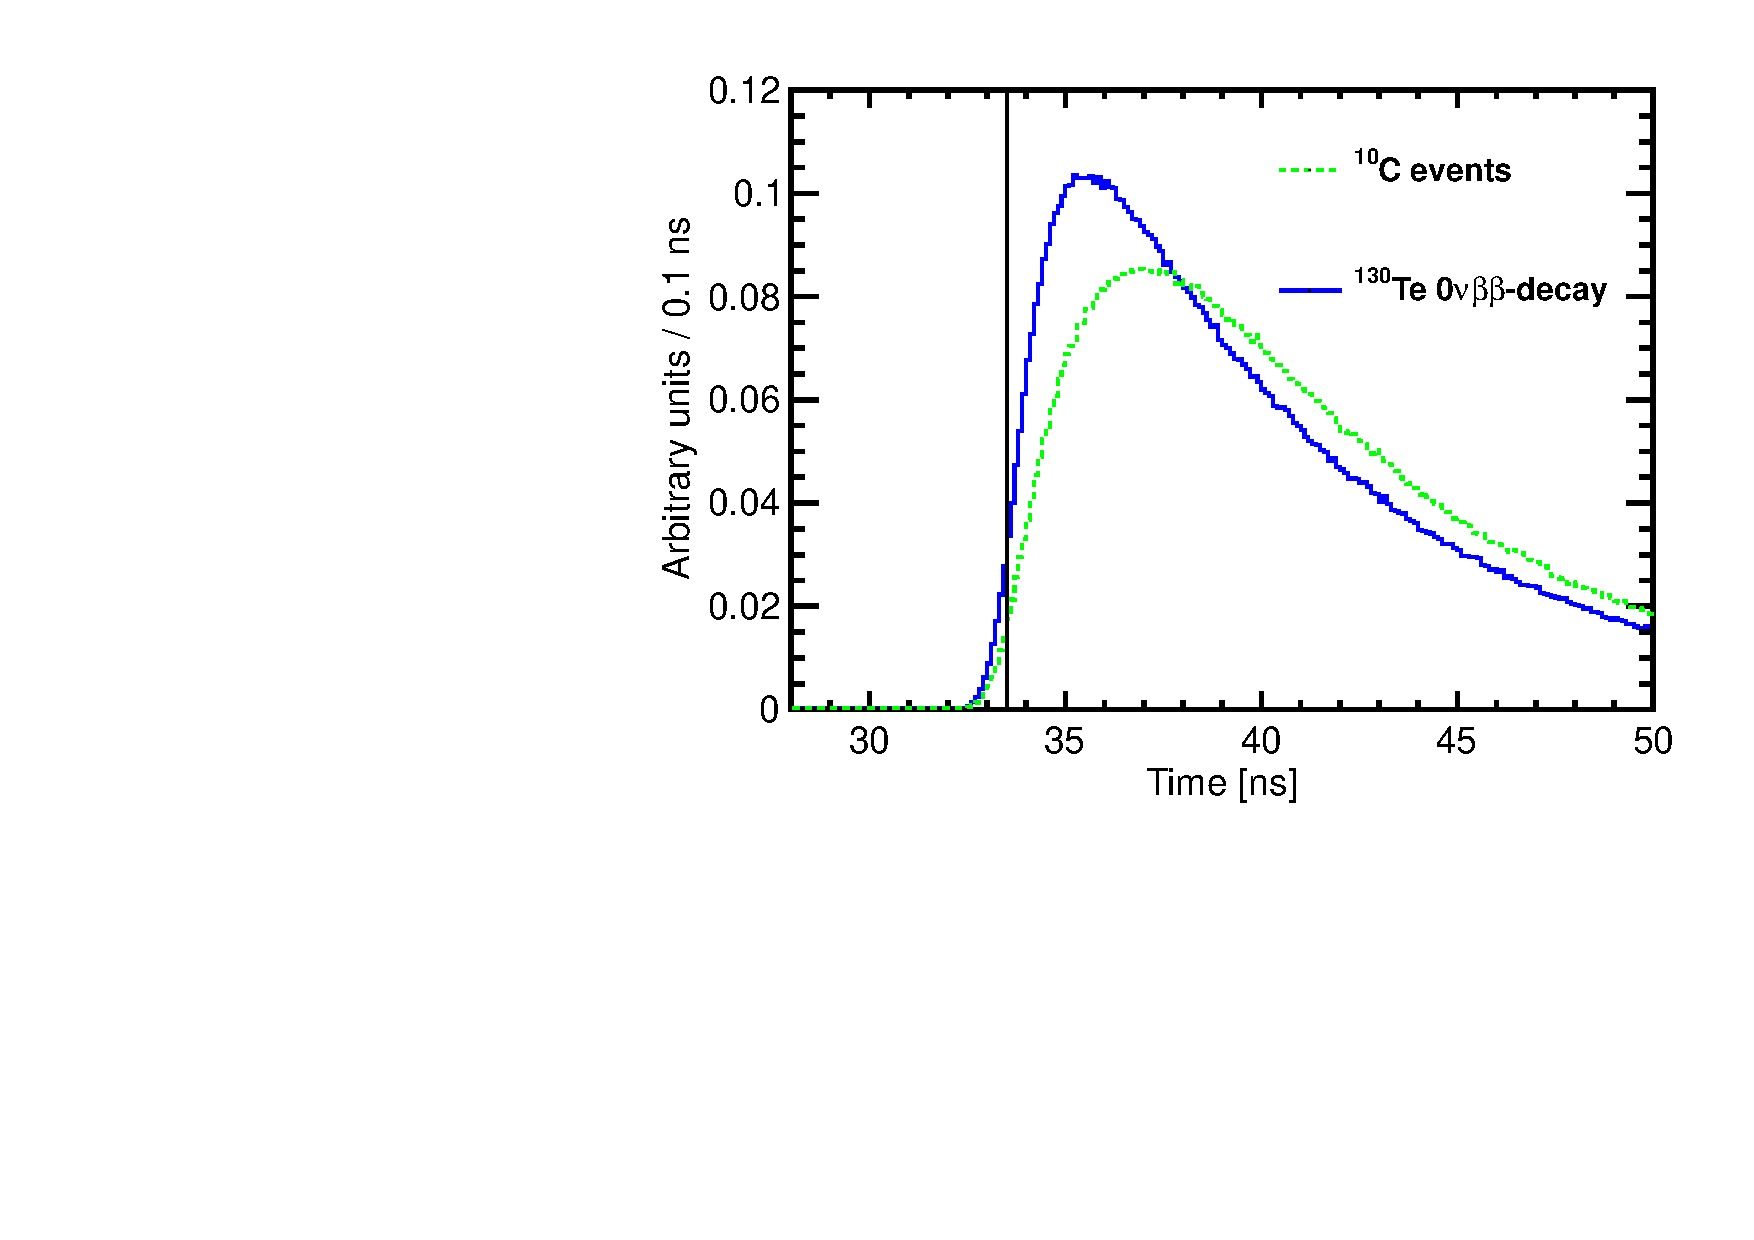
\includegraphics[angle=0,width=0.45\textwidth]{plots/hT_C10.pdf}
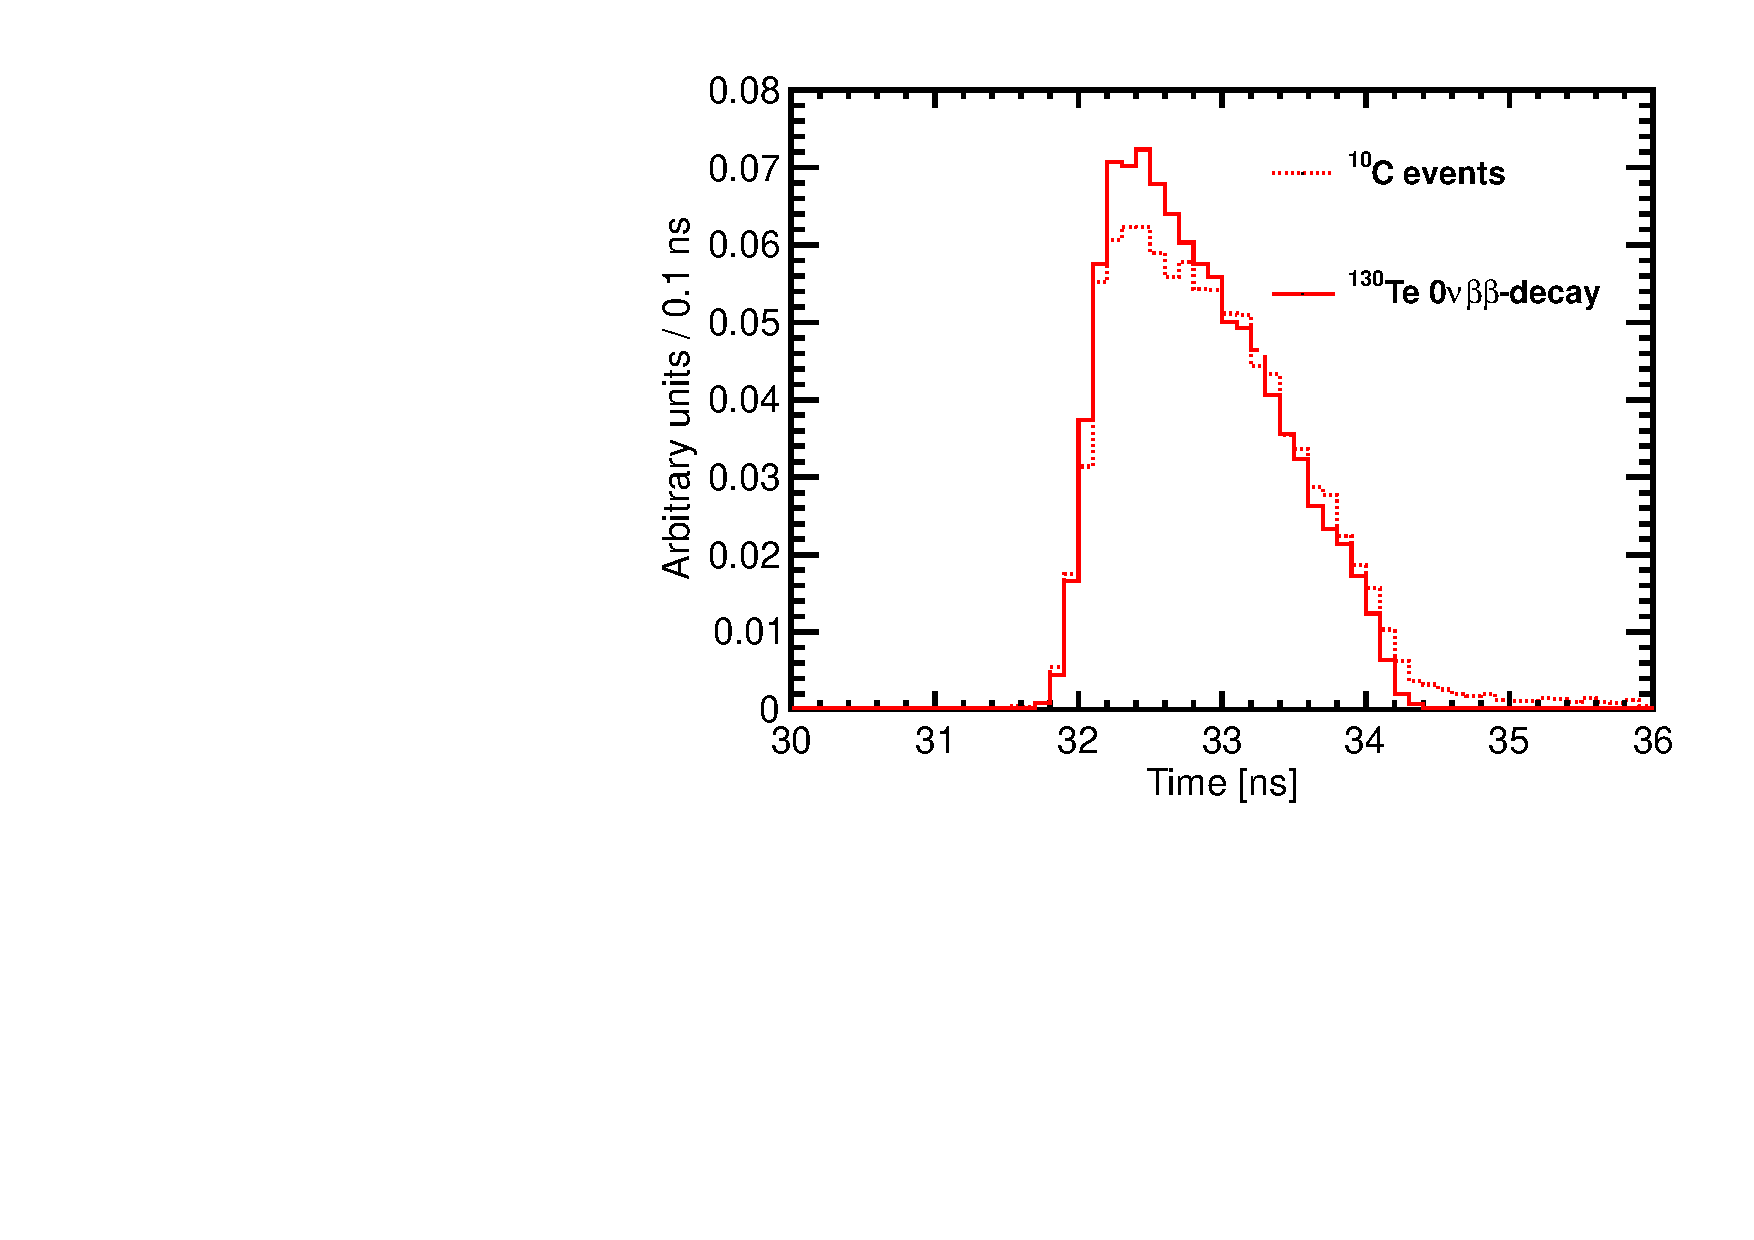
\includegraphics[angle=0,width=0.45\textwidth]{plots/hTche_C10.pdf}
\caption{Photo-electron (PE) arrival times after application of the photo-detector transit time spread (TTS) of 100~ps for the simulation of 1000 $\vbb$-decay events of $\Te$ (solid lines) and $\Cten$ (dotted lines) events at the center of the detector. All distributions are normalized for shape comparison. {\bf Absolute number of PEs per event depends on the total energy deposited in the detector. Figure~\ref{fig:Edep_C10} shows energy deposited in the detector in $\Cten$ events.} (Left) Scintillation PEs arrival time. The black vertical line illustrates a time cut at 33.5 ns. (Right) Cherenkov PEs arrival time.}
\label{fig:Arrival_time_C10}
\end{figure}

We note that 98\% of $\Cten$ decays through the excited state of $\Bten$(718) that has a half-life time of $\sim$1~ns. Therefore majority of $\Cten$ events have a prompt positron accompanied by a delayed 0.718~MeV gamma. This delayed gamma affects PEs arrival time distribution. Figure~\ref{fig:Arrival_time_C10} shows shape comparison of PEs arrival time distribution between $\Te$ $\vbb$-decay and  $\Cten$ events. Time profile of the scintillation photons can be used to separate signal from $\Cten$ events.


\begin{figure}[htb]
\centering
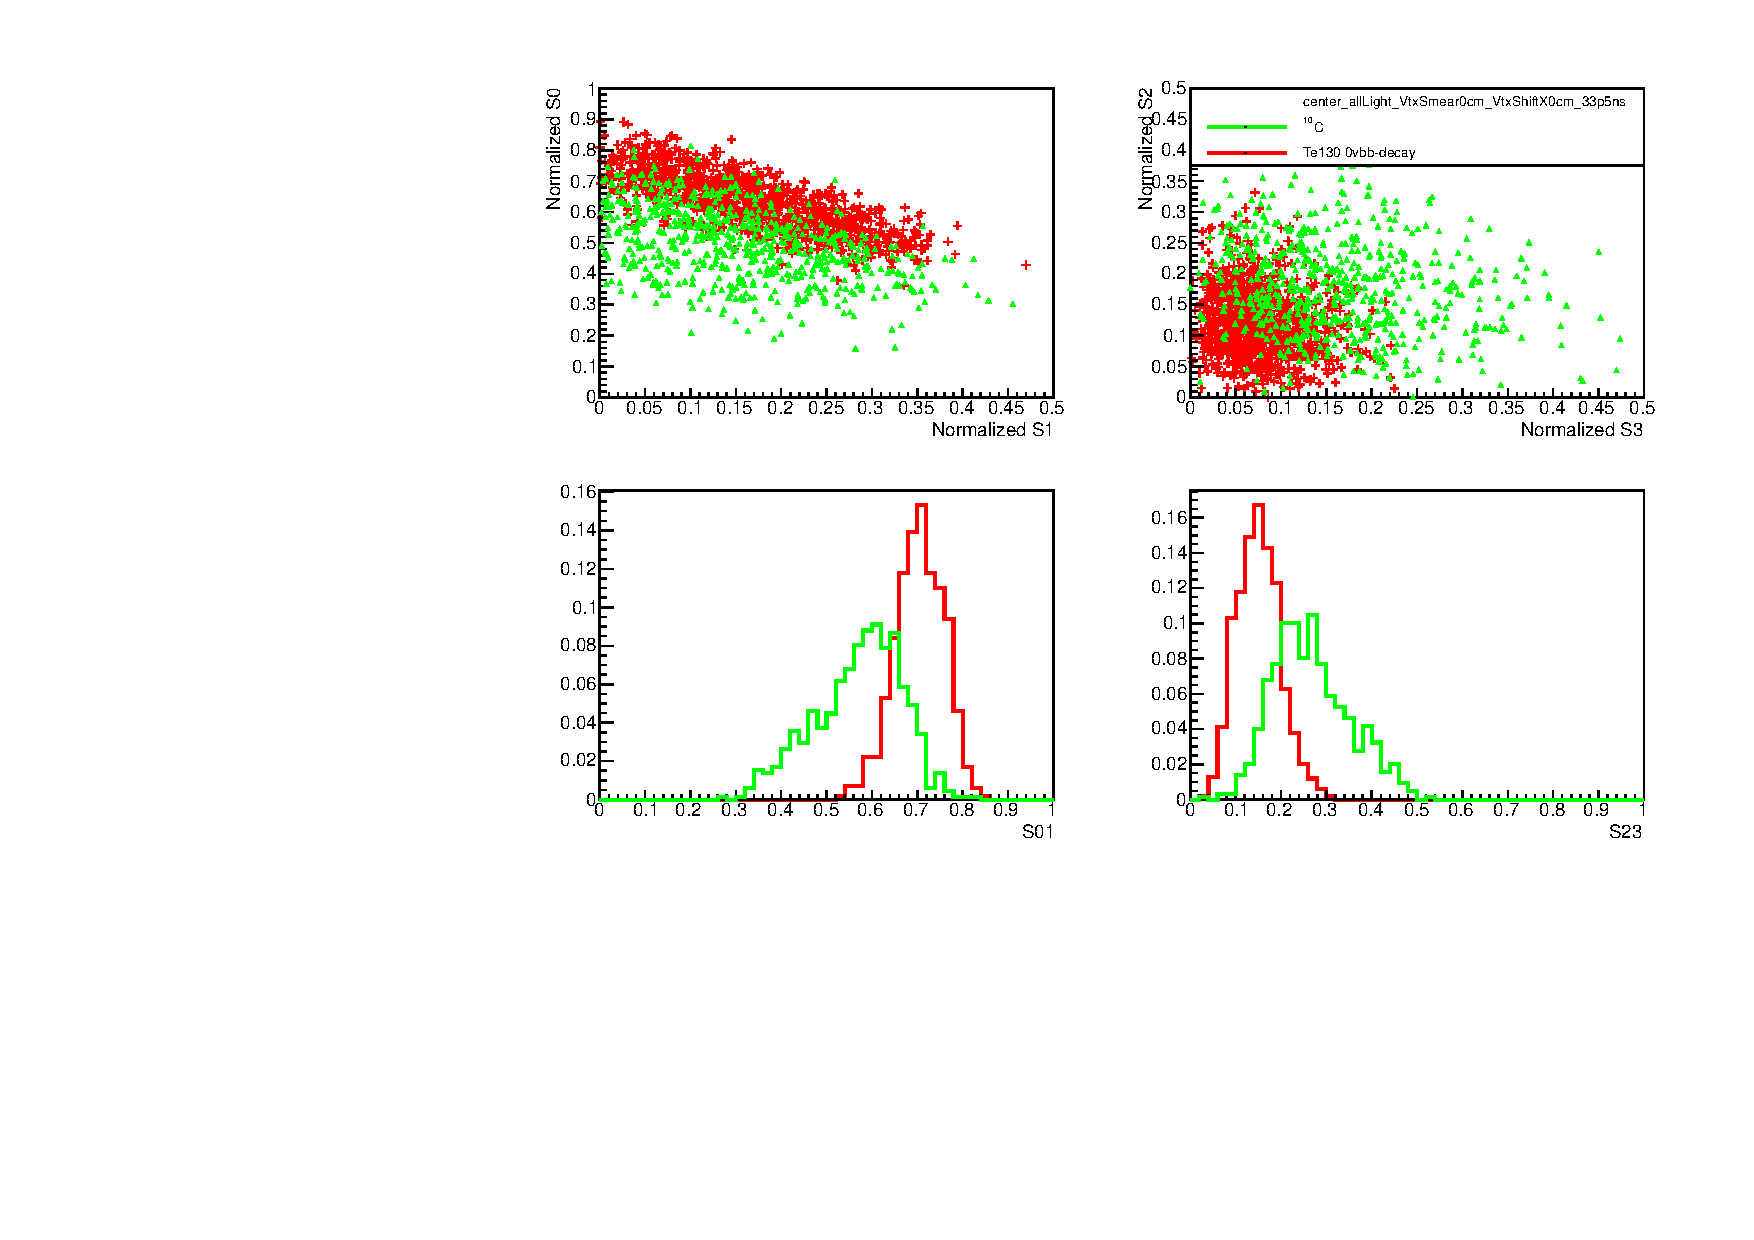
\includegraphics[angle=0,width=0.95\textwidth]{plots/hSLPlots_C10_allLight_VtxSmear0cm_VtxShiftX0cm_33p5ns_center.pdf}
\caption{Spherical harmonics comparison between $\Te$ $\vbb$-decay signal (Q$=$2.529~MeV) (red) and $\Cten$ solar neutrinos background (blue) for 1000 simulated events originated at the center of the sphere. $\Cten$ with energy deposition between 2.1~MeV and 2.9~MeV are considered. Perfect vertex reconstruction - true vertex position is used. Time cut of 33.5~ns on the photon arrival time is applied. (Top left) S$_0$ versus S$_1$ scatter plot. (Top right) S$_2$ versus S$_3$ scatter plot. (Bottom left) Distribution of the S$^{C10}_{01}$ variable calculated for signal (red) and background (green). (Bottom right) Distribution of the S$^{C10}_{23}$ variable calculated for signal (red) and background (green).}
\label{fig:SL_C10_33p5ns_center}
\end{figure}


Comparison of spherical harmonics is shown in Fig.~\ref{fig:SL_C10_33p5ns_center}. $\Cten$ events are generated at the center of the detector. True vertex position is used to apply a 33.5~ns time cut to select photons for the spherical harmonics analysis. The separation is seen in S0 vs S1 and S2 vs S3 scatter plots. We project both scatter plots to a line that gives maximum separation (two bottom panels in Fig.~\ref{fig:SL_C10_33p5ns_center}).

%\section{$\vbb$-decay vs backgrounds from Th and U series}

\begin{thebibliography}{00}
\bibitem{Directionality} C.~Aberle et al. JINST 9 P06012.
\bibitem{SNOp_paper} A good ref to SNO+ backgrounds description.
\end{thebibliography}

\end{document}
